\section{Simulation}
\label{section:simulation}

\subsection{Injection via BTP}
As the beam is injected through the BTP transfer line to the PS ring, it passes through the stray fields of the PR.BHT41 T-type MU magnet. The beam traverses mostly through the defocusing half part and feels a non-linear increase in the gradient up to the nominal value in the central orbit; see Fig.~\ref{fig:injection_btp}. Once through MU41, the beam is deflected by the injection septum magnet (PI.SMH42) towards the central orbit. Immediately downstream of the septum, a Secondary Emission Grid (PI.BSG42) is available to measure the position and size of the beam.
\\
\\
\begin{figure}[!htb]
   \centering
   \includegraphics*[width=0.7\columnwidth]{01_Introduction/images/injection_tracking.png}
   \caption{Tracking through MU41 T-type at \SI{2}{GeV}.}
   \label{fig:injection_btp}
\end{figure}

To test the model, measurements of beam position and size on PI.BSG42 were collected as the current provided by the main power supply (POPS) to the MUs was varied. As expected, an increasing current shows that the transverse position of the beam is bent closer towards the inside of the ring by the stronger stray field. Measurements were compared with simulations that tracked a single particle through the \SI{2}{GeV} T-type field map presented in Fig.~\ref{fig:injection_btp_transverse_position}. The tracking simulation overestimates the effect of the stray field because the magnetic model does not include the mu-metal shielding wrapped around the injection vacuum pipe. As expected, no deviation was observed in the vertical plane.

\begin{figure}[!htb]
   \centering
   \includegraphics*[width=0.7\columnwidth]{01_Introduction/images/injection_measurement.png}
   \caption{Measurements of the BT3 BTP PS kick response as a function of POPS at PI.BSG42 compared with the OPERA tracking model.}
   \label{fig:injection_btp_transverse_position}
\end{figure}

The current implementation of the stray field in the \mbox{MAD-X}\cite{noauthor_mad_nodate} model is carried out as a sequence of Multipole Field Components (MFC model) expanded along the reference trajectory. A simplified approach with the field components extracted on an injected trajectory assumed as a straight line was compared with the measurements in Fig.~\ref{fig:injection_btp_beam_size}, where the beam size at PI.BSG42 is plotted as a function of the POPS current. We find good agreement in the horizontal plane but a mismatch in the vertical plane. Similar MFC models for injection and extraction have been created using a Taylor series of the multipole components of the magnetic field about the curved trajectory of the reference particle and will be discussed in section \ref{BTP Stray Elements}.

\begin{figure}[!htb]
   \centering
   \includegraphics*[width=0.7\columnwidth]{01_Introduction/images/injection_measurement_beam_size.png}
   \caption{Measurements of the BT3 BTP PS beam size as a function of POPS at PI.BSG42 compared with the MFC model.}
   \label{fig:injection_btp_beam_size}
\end{figure}

%\subsection{Extraction to the East Area}
%The beam extracted to the East Area is significantly affected by stray fields in multiple main units because the slow extracted trajectory at high energy has a much shallower angle than at injection. As presented in Fig.~\ref{fig:stray field gradients}, the difference in the gradient of MU62 is striking in that the sign of the gradient flips and triples in amplitude. As a result, an increase in the horizontal beam size is expected at the exit of MU62. It is not understood why this magnet was not shimmed in the past to help reduce the effect of the stray field (perhaps because they would significantly impact the central orbit \cite{Zickler:private}), but it is undoubtedly the cause of the optics discrepancy observed during commissioning of the East Area transfer lines in 2021 \cite{huschauer:ipac22-mopost006}.

%\begin{figure}[!htb]
%   \centering
%   \includegraphics*[width=0.7\columnwidth]{01_Introduction/images/gradient_stray_field.png}
%   \caption{Gradient seen by the slow extracted beam in the stray field of the few last MUs's focusing half-unit.}
%   \label{fig:stray field gradients}
%\end{figure}



\subsection{Multipole Field Components (MFC model)}
\label{BTP Stray Elements}

The BTP line has an old model (prior to 2021) that is composed of 233 thin multipole inserted at the end of the transfer line. This model served as an example and foundational framework for building further Multipole Field Component (MFC) models. By examining the structure and implementation of the BTP model, we were able to understand how thin multipoles can be effectively used to simulate complex magnetic fields along a transfer line. This knowledge was then applied to develop more accurate and detailed MFC models for other sections of the PS, including the main units and extraction lines. The model can be accessed via the following links:

\begin{itemize}
    \item \href{https://gitlab.cern.ch/acc-models/acc-models-tls/-/blob/2021/psb_extraction/btp/BTP.ele}{BTP.ele}
    \item \href{https://gitlab.cern.ch/acc-models/acc-models-tls/-/blob/2021/psb_extraction/btp/BTP.seq}{BTP.seq}
\end{itemize}



\subsection{Multipole Field Components Computation}

The magnetic field \( B_y \) can be expressed as:

\[
B_{y}(x,y) = B_{0} + B_{1}x + B_{2}\frac{1}{2}(x^{2}-y^{2}) + B_{3}\frac{1}{6}(x^{3}-3xy^{2})
\]

where the coefficients \( B_i \) are given by:

\[
B_{i} = K_{i}B\rho
\]

In the old BTP model, the coefficients \( K_{0}, K_{1}, K_{2}, \) and \( K_{3} \) are used. The relationship for \( K_{0} \) is:

\[
K_{0}L = \frac{B_{0}L}{B\rho}
\]

where 

\[
L = \frac{\text{totalLength}}{\# \text{ elements}}
\]

To extract the pure \( K_{0} \), we divide by \( L \):

\[
K_{0} = \frac{B_{0}}{B\rho}
\]

For tracking, we obtain the field components and divide by \( B\rho \):

\[
B_{0} = K_{0}B\rho
\]

\[
K_{0} = \frac{B_{0}}{B\rho}
\]

The \( K_{1} \) coefficient is computed using two point that are computed transversely to the track and the relationship:

\[
K_{1} = \frac{\frac{\Delta B_{y}}{\Delta x}}{B\rho}
\]

The \( K_{0}L \) component as a function of \( s \) is shown as follows:

\begin{figure}[H]
\centering
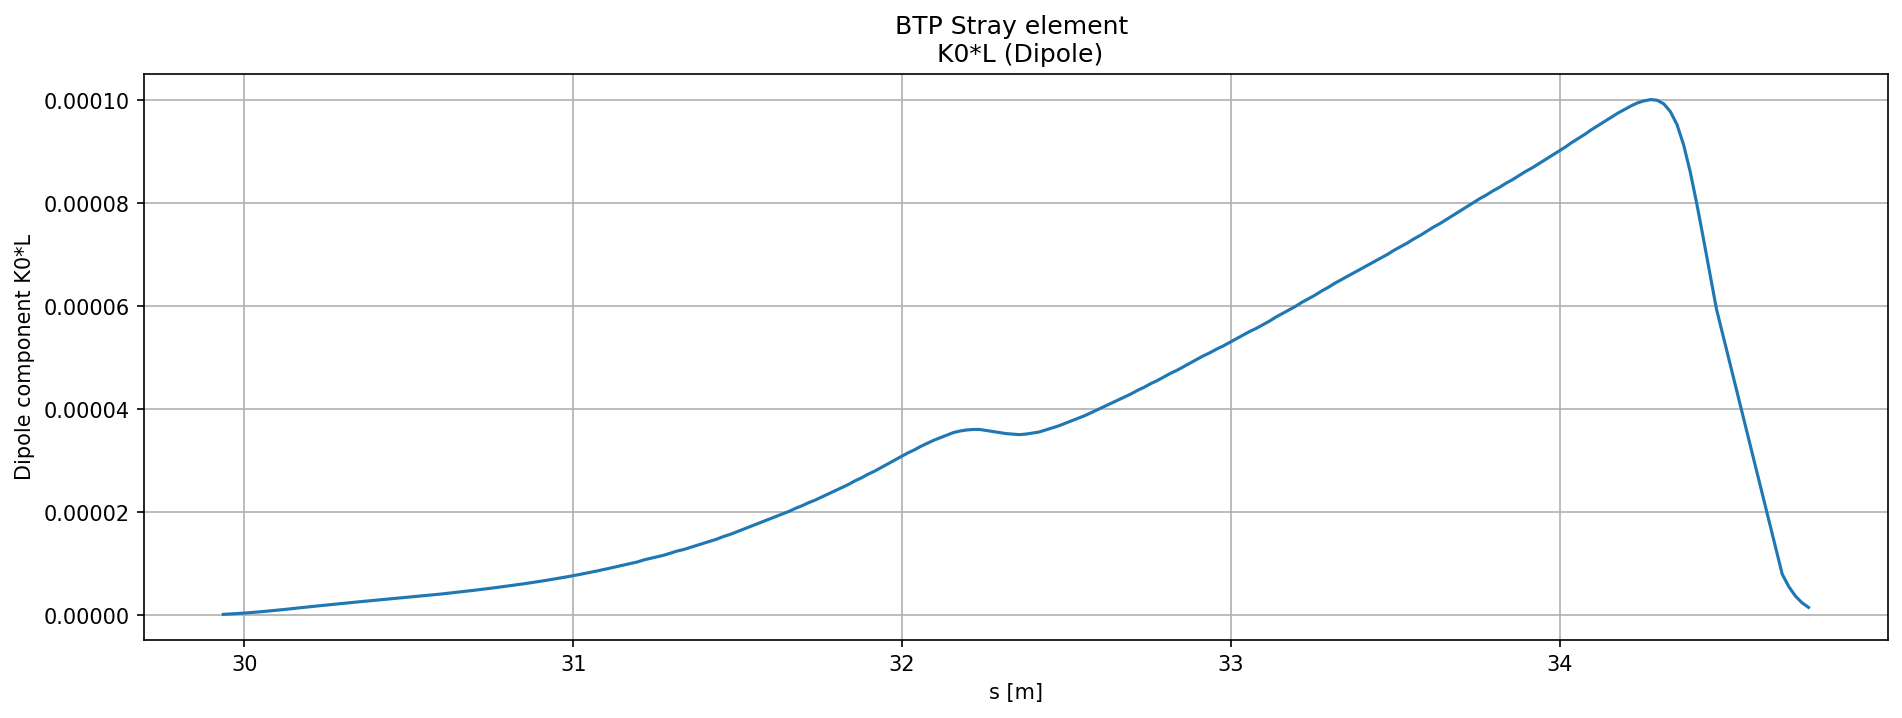
\includegraphics[width=1.0\textwidth]{02_Simulation/images/BTP_old_model_stray.png}
\caption{BTP Stray Element - Reference Model.}
\label{fig:transfer_matrix_1}
\end{figure}


The goal is to create a multi-component model similar to the old BTP model, starting with the BTP line to compare with the old model and then expanding to different injection and extraction lines that pass through stray fields. The first step is to launch particles on the reference track, track them in the stray field magnetic field, and probe the B-field perpendicular to the track. This process is illustrated in Figure \ref{fig:mcp_track}. The transverse B-field along the injection track is shown in Figure \ref{fig:mcp_track_2}. 

Next, a 4th-order polynomial is fitted for every position along the injection line, i.e., along different z positions in meters, as depicted in Figure \ref{fig:fit_bfield}. The results from these polynomial fits are then used to compare different multipole components of the magnetic field.

Figures \ref{fig:mcp_dipole} through \ref{fig:mcp_octupole} show the comparisons of the BTP stray multipole components: K0 (Dipole), K1 (Quadrupole), K2 (Sextupole), and K3 (Octupoles), respectively. These comparisons help validate the accuracy and detail of the multipole components from the new tracking script against the old BTP model.

\begin{figure}[H]
\centering
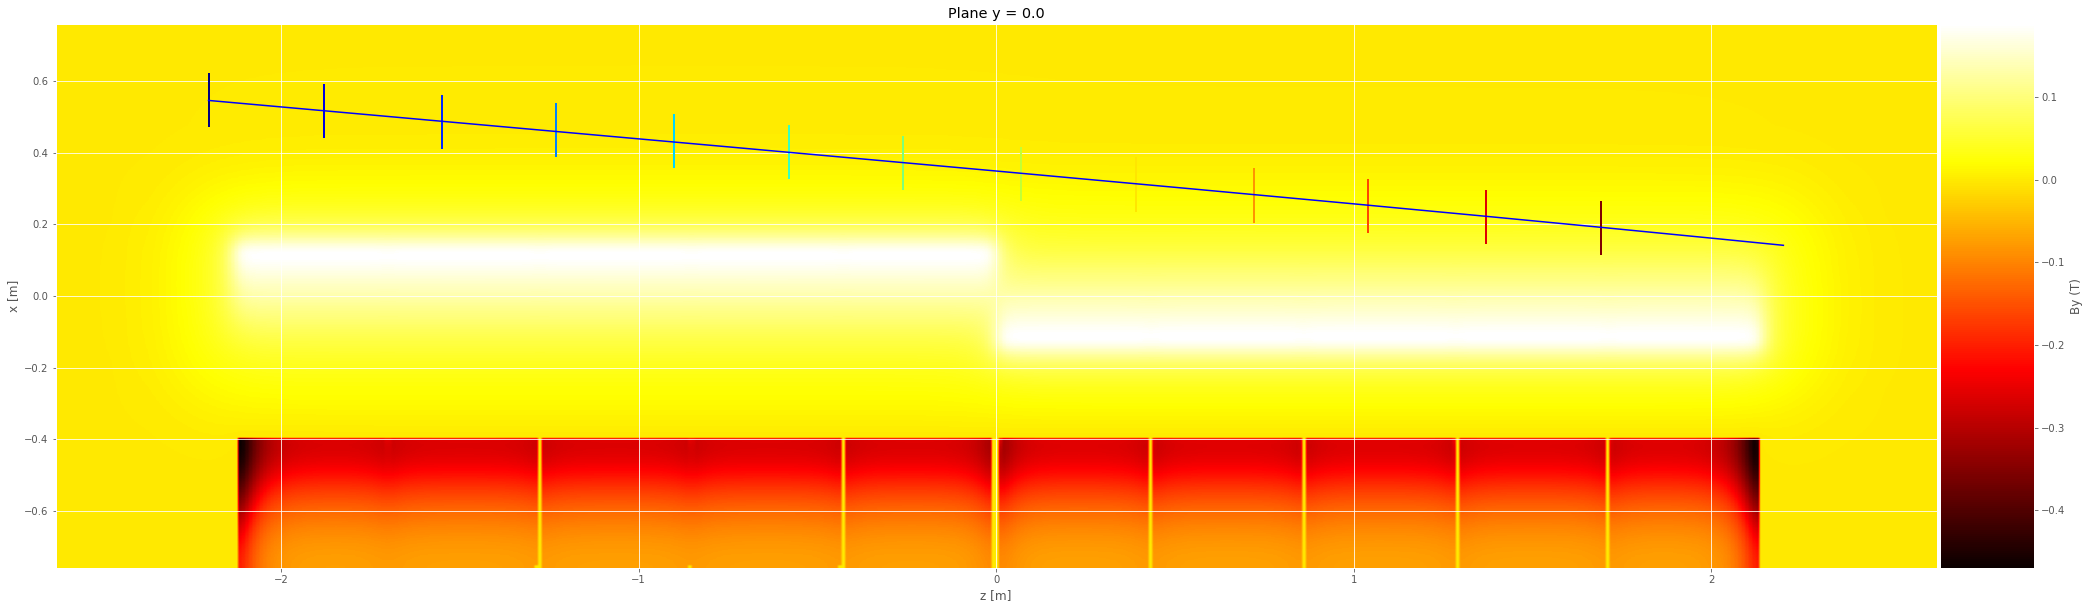
\includegraphics[width=1.0\textwidth]{02_Simulation/images/MCP_track.png}
\caption{Particle tracking through the magnetic field at injection in the PS via the BTP line. Note: this plot shows a old version of the script where the field is not computed transversely to the particle trajectory (lines are vertical) but this has been fixed in the following computations.}
\label{fig:mcp_track}
\end{figure}

\begin{figure}[H]
\centering
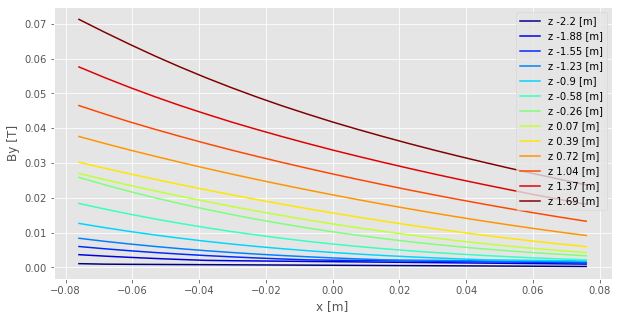
\includegraphics[width=1.0\textwidth]{02_Simulation/images/MCP_track_2.png}
\caption{Transverse B-field along the injection track. One notices the increase in magnetic field as we increase z and move towards the magnet.}
\label{fig:mcp_track_2}
\end{figure}

\begin{figure}[H]
\centering
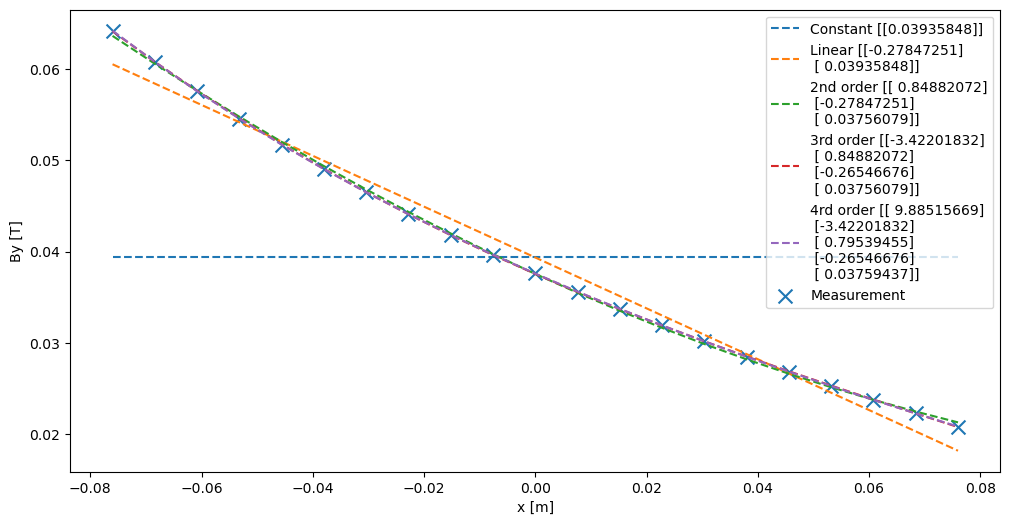
\includegraphics[width=1.0\textwidth]{02_Simulation/images/fit_of_bfield.png}
\caption{Polynomial Fits of \( B_y \) vs. \( x \) for Different Orders.}
\label{fig:fit_bfield}
\end{figure}

\begin{figure}[H]
\centering
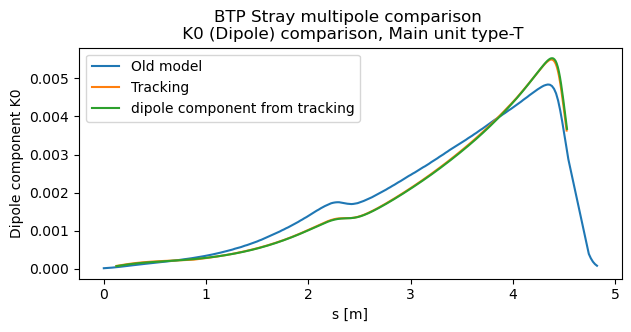
\includegraphics[width=0.7\textwidth]{02_Simulation/images/mcp_dipole.png}
\caption{BTP Stray multipole comparison, K0 (Dipole) comparison, main unit type-T.}
\label{fig:mcp_dipole}
\end{figure}

\begin{figure}[H]
\centering
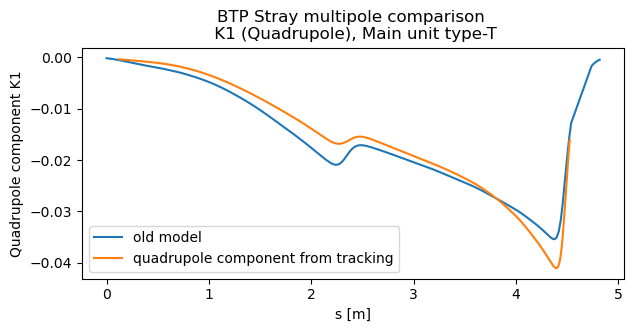
\includegraphics[width=0.7\textwidth]{02_Simulation/images/mcp_quadrupole.png}
\caption{BTP Stray multipole comparison, K1 (Quadrupole) comparison, main unit type-T.}
\label{fig:mcp_quadrupole}
\end{figure}

\begin{figure}[H]
\centering
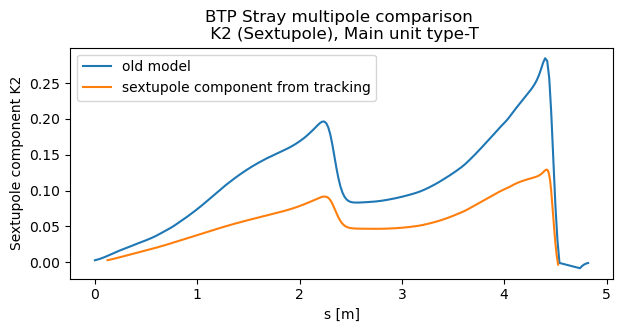
\includegraphics[width=0.7\textwidth]{02_Simulation/images/mcp_sextupole.png}
\caption{BTP Stray multipole comparison, K2 (Sextupole) comparison, main unit type-T.}
\label{fig:mcp_sextupole}
\end{figure}

\begin{figure}[H]
\centering
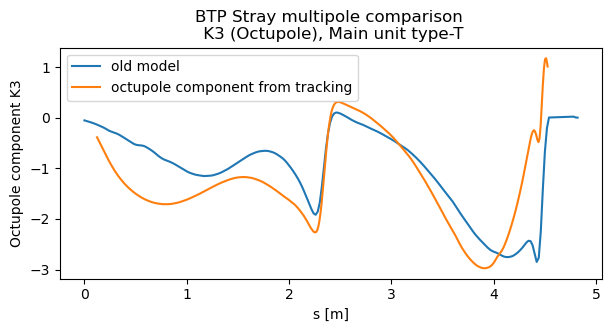
\includegraphics[width=0.7\textwidth]{02_Simulation/images/mcp_octupoles.png}
\caption{BTP Stray multipole comparison, K3 (Octupoles) comparison, main unit type-T.}
\label{fig:mcp_octupole}
\end{figure}

The code accurately generates MCP models along the s-dimension (aligned with the particles' trajectory) and transversely along the bending track. For small angles, the variation in the dipole component between the z and s directions can be considered negligible.

\subsection{Multipole field component in MU62}

This section describes the creation of the Multiple Field Component (MFC) within the MU62 main unit, the critical magnet through which the particle beam traverses during extraction to the East Area. The \href{https://gitlab.cern.ch/eljohnso/acc-models-tls-eliott-fork/-/blob/EliottBranch/ps_extraction/east-fast-extraction/mfc_mu62.ipynb}{Notebook: MFC MU62} was used to develop the MFC in MU62, using a \SI{24}{\giga\electronvolt\per\clight} beam. Figure \ref{fig:track_mu62_2} illustrates the particle track through the stray field of MU62. The initial launching coordinates of the reference particle were \SI{0.132}{\meter} and \SI{0.0139}{\radian}. The field was probed transversely at discrete s-steps along the particle trajectory inside the vacuum pipe, which has a total aperture width of \SI{70}{\milli\meter}. For each point in the track, the $B_{y}$ field perpendicular to the track was recorded, and a third-order polynomial fit of $B_{y}$ as a function of $x_{\perp}$ was performed.

$$ \alpha = - tan^{-1}\left(\frac{ x_{i}-x_{i-1} } {z_{i}-z_{i-1}} \right)$$

$$ B_{y} = \begin{bmatrix}  
x_{center} + x_{offset}\cdot cos(\alpha_{deflection}) \\  
0 \\
z_{center} + x_{offset}\cdot sin(\alpha_{deflection})
\end{bmatrix} $$


\begin{figure}[H]
\centering
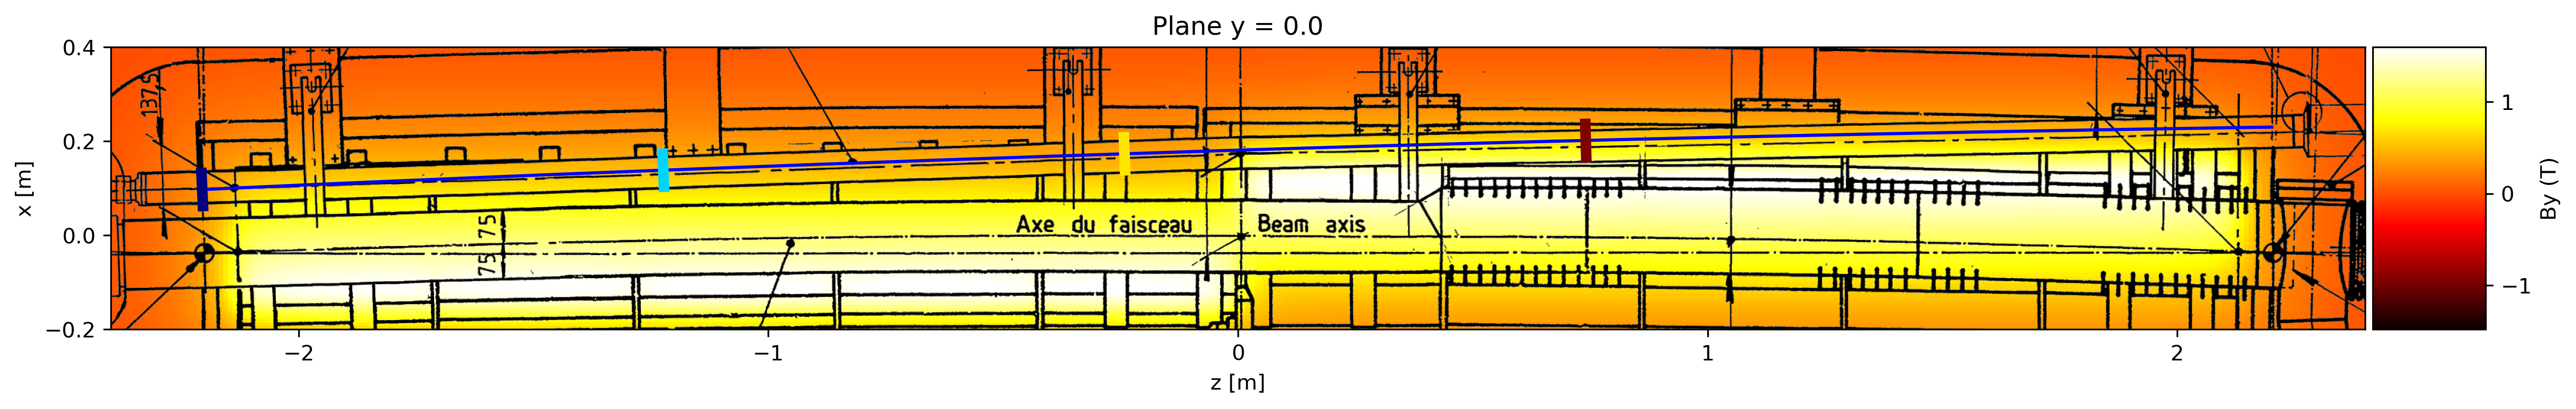
\includegraphics[width=1.0\textwidth]{02_Simulation/images/track_mu62_2.png}
\caption{Tracking of the proton beam in MU62 with example location of MFC sampling}
\label{fig:track_mu62_2}
\end{figure}

\begin{figure}[H]
\centering
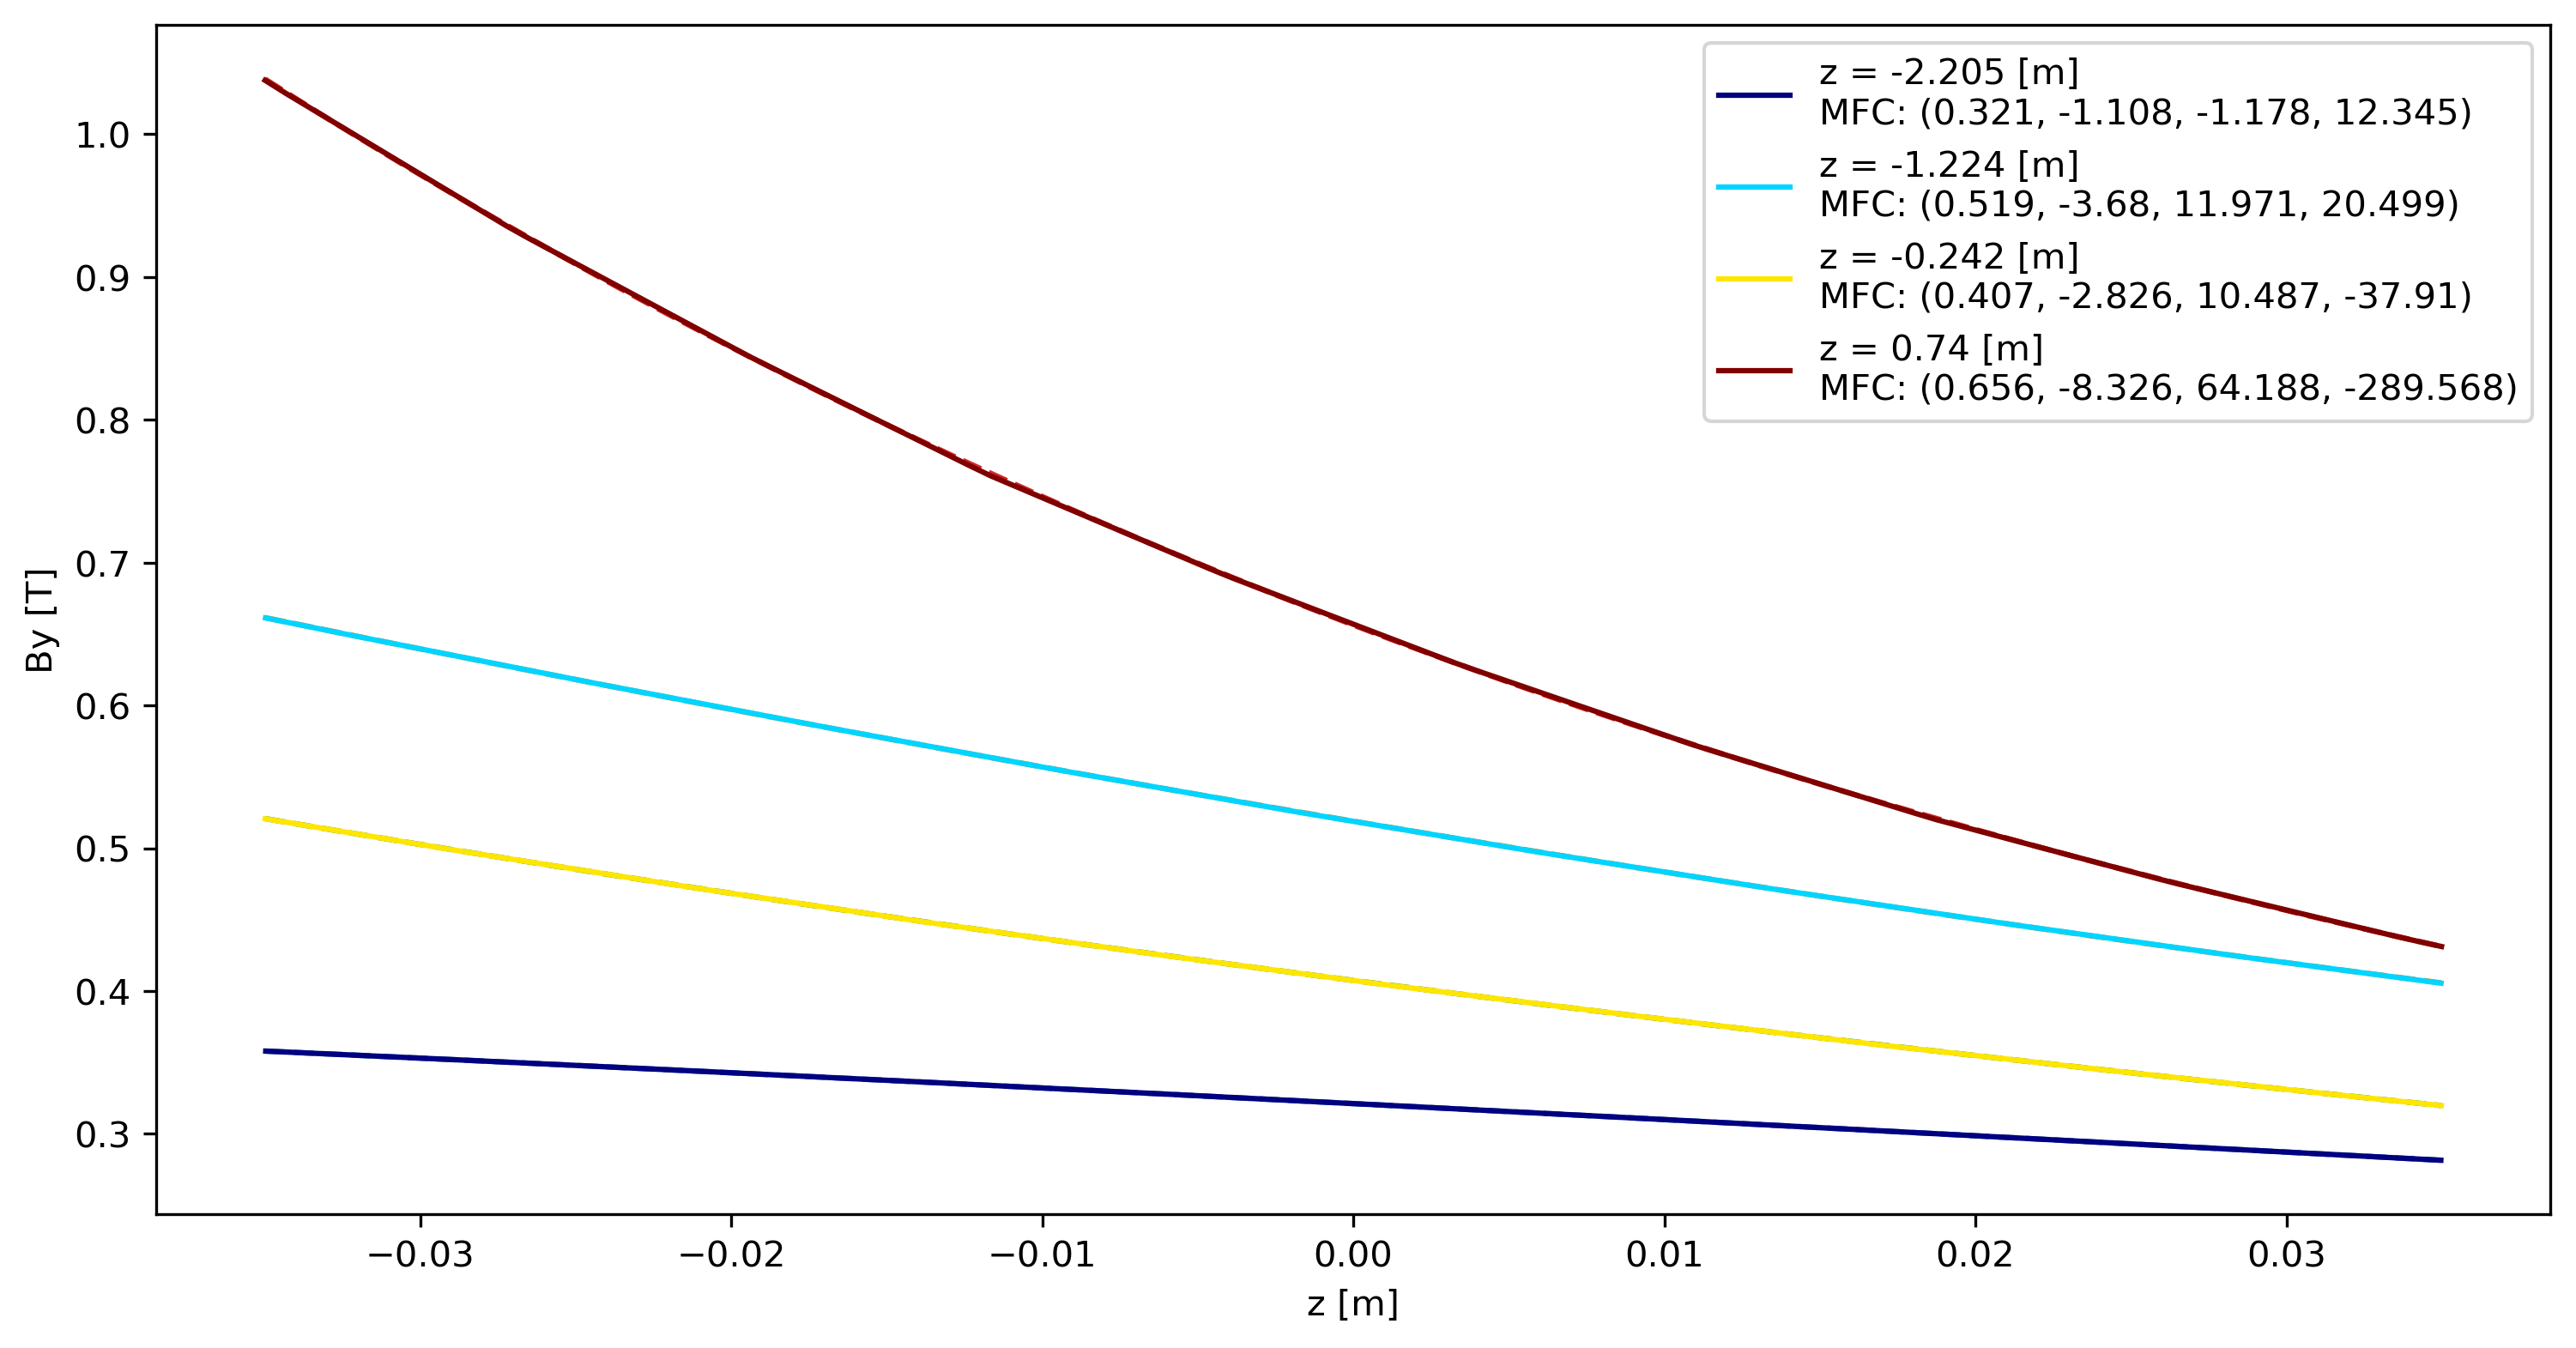
\includegraphics[width=0.7\textwidth]{02_Simulation/images/track_mu62_2_mfc.png}
\caption{Tracking of the Proton Beam in the Transverse Dipoles Component of MU62 and polynomial fit to create the MFC. The x-axis label should be $x_{T}$ [m]}
\label{fig:track_mu62_2_mfc}
\end{figure}

Full tracking with fine sampling along the beam line gives us the following MFC shown in Fig. \ref{fig:mfc_mu62}.

\begin{figure}[H]
\centering
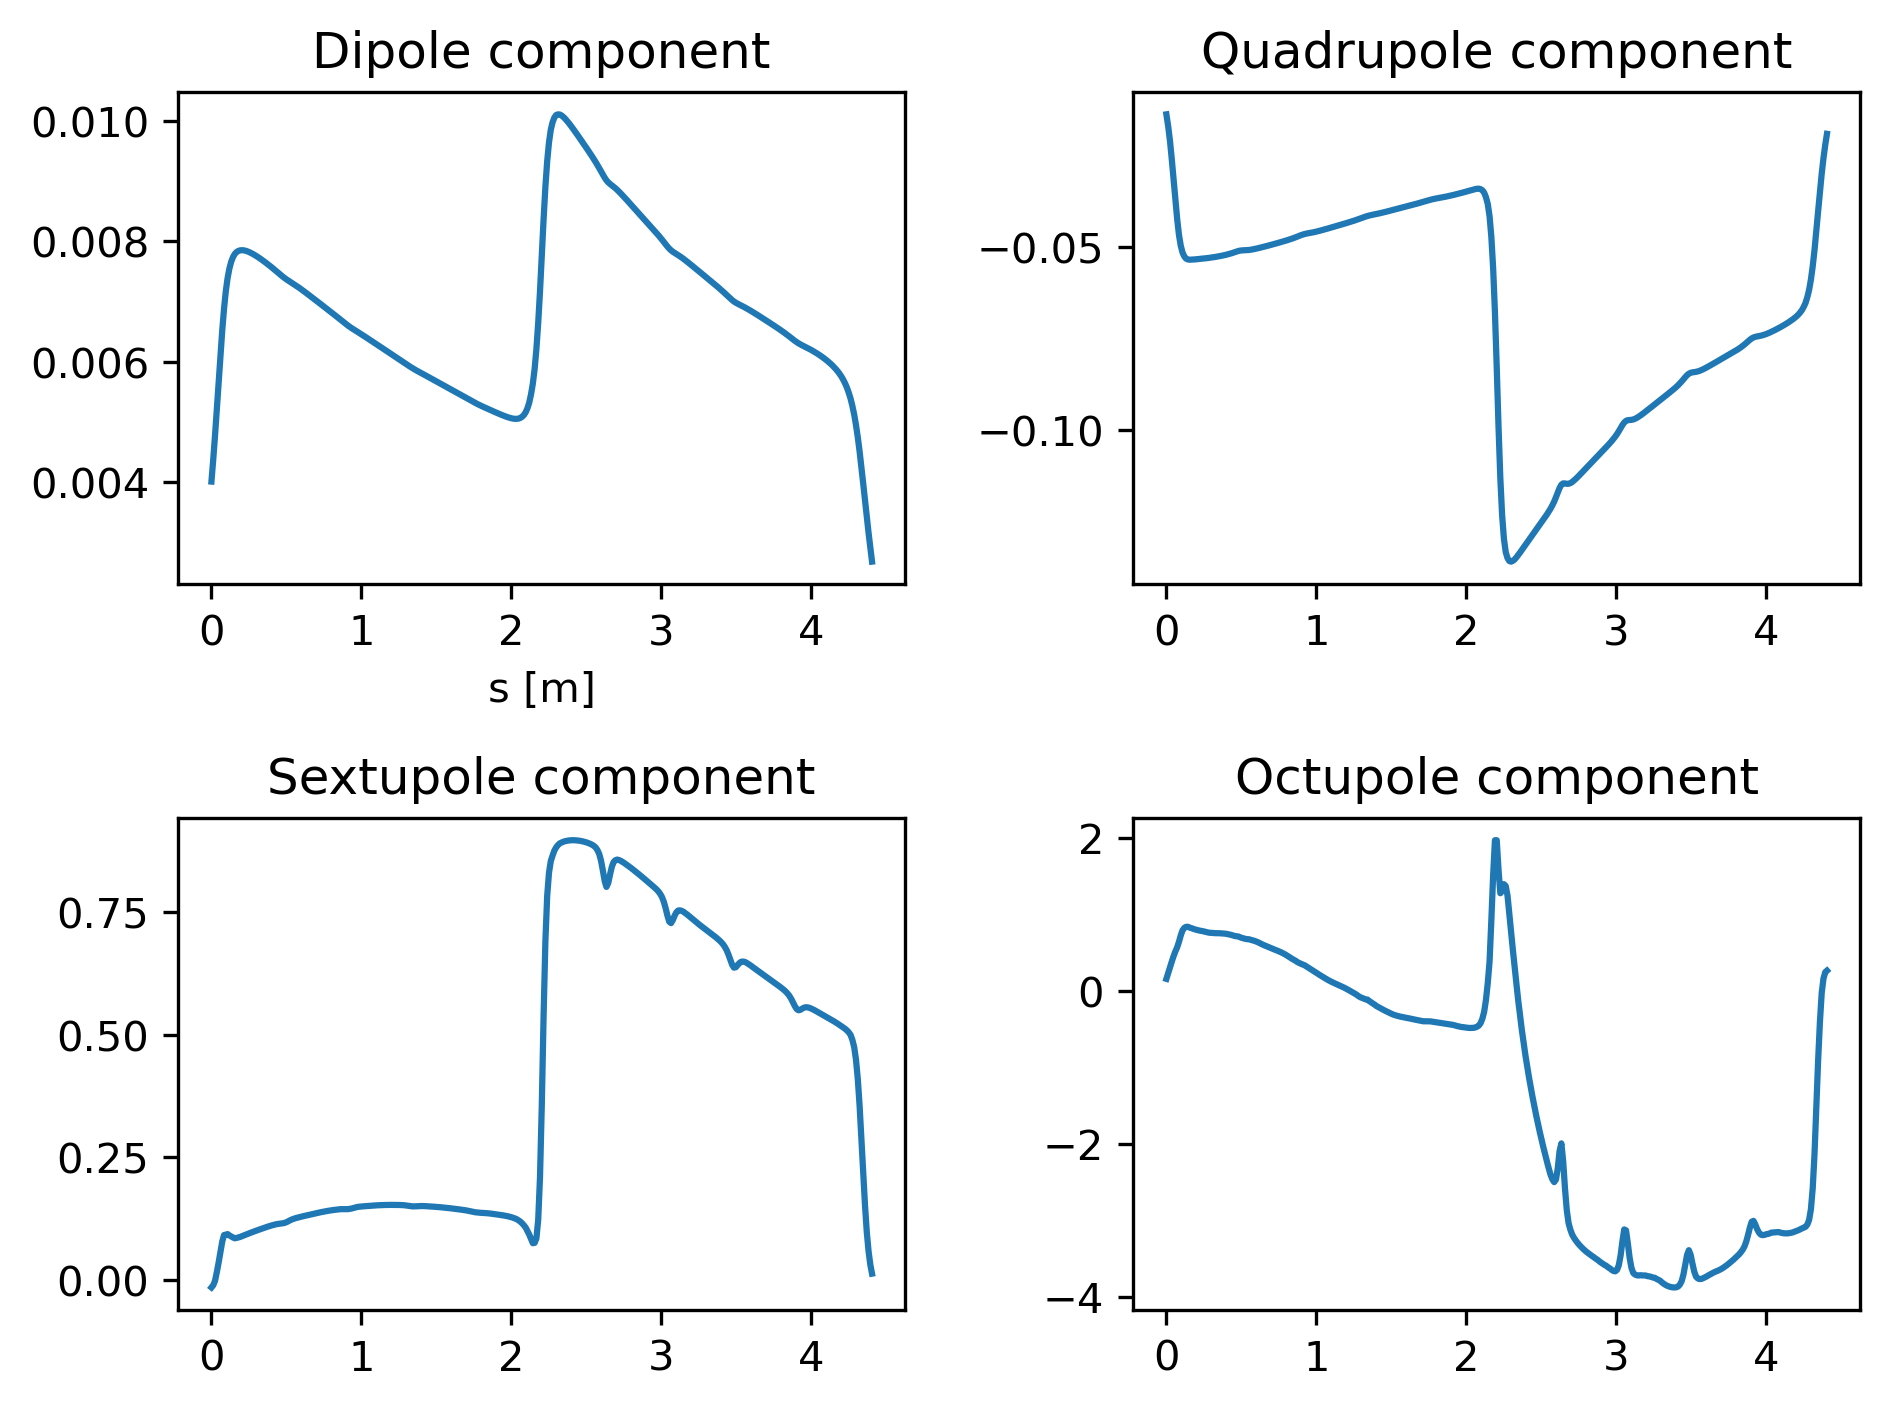
\includegraphics[width=0.7\textwidth]{02_Simulation/images/mfc_mu62.png}
\caption{Fine sampling of the magnetic field in MU62 and expansion into MFC.}
\label{fig:mfc_mu62}
\end{figure}

Theses MFC components can be exported to a file to be used in MAD-X as multipoles. The format for the \texttt{.ele} file is as follows:

\begin{lstlisting}
stray1 : multipole, knl:={2.11E-07,-3.11E-06,5.25E-05,-0.001056026};
stray2 : multipole, knl:={2.78E-07,-4.03E-06,6.74E-05,-0.001303161};
stray3 : multipole, knl:={3.54E-07,-5.09E-06,8.47E-05,-0.001548501};
\end{lstlisting}

When exporting the multipole component, it is necessary to multiply by the length of the multipole element, i.e.,:

\[
\frac{L_{\text{Total}}}{l_{\text{element}}}
\]

The format for the \texttt{.seq} file is as follows:

\begin{lstlisting}
stray1, at = 29.9366067;
stray2, at = 29.9566067;
stray3, at = 29.9766067;
\end{lstlisting}

\subsection{Initial condition in F61D}

To test the accuracy of the MFC model, the F61D transfer line from the PS to the East Dump was chosen as it can be used extensively for Machine Development (MD) studies as it contains a BTV for beam size measurement and three quadrupoles for optics. It can also be operated in parallel to the operational beams with no impact on them. A more detailed description of the line can be found in section \ref{Quadrupole Scan}.
\\
\\
The initial condition of the F61D transfer line were found using the twiss parameters from the PS Ring slow extraction \href{https://gitlab.cern.ch/eljohnso/acc-models-tls-eliott-fork/-/blob/EliottBranch/ps_extraction/east-fast-extraction/Check%20scripts/slow_extraction_trajectory_maptrack_inital_conditions.ipynb}{script}. The beam envelope was extracted using a pycollimate simulation and retrieving the four particles marking the edge of the extracted separatrix, see Fig. \ref{fig:init_pycollimate}.

\begin{figure}[H]
\centering
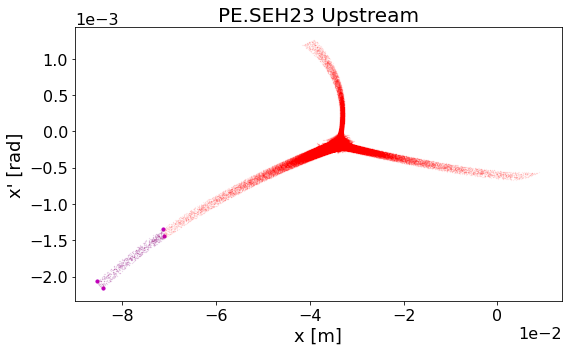
\includegraphics[width=0.7\textwidth]{02_Simulation/images/init_pycollimate.png}
\caption{Distribution of particles in the PS and the four particles at the extremity of the separatrix used as beam envelope.}
\label{fig:init_pycollimate}
\end{figure}

The tune of the PS was match to be on resonance and the chromaticity match to measurement from 12.11.2021 (Qxp=-1.239, Qyp=0.242). These four particles were tracked during their last turn before being extracted in the PS with the electrostatic septum and the magnetic septa on. The strength of the electrostatic septum (SEH23) was determined by applying a voltage of \SI{-177}{\kilo\volt} across a gap of \SI{15.11}{\milli\metre}, resulting in an electric field of \SI{11.708}{\mega\volt\per\metre}. Given an effective length of \SI{0.8}{\metre}, the resulting strength was calculated as $\theta_{SEH23} = \arctan \left( \frac{|\mathbf{E}| \cdot \text{effective length}}{p \cdot \beta \cdot 10^9} \right)$, and incorporated into the MAD-X input as \texttt{kPESEH23}.
\\
\\
For the magnetic septa, the strength of SMH57 was derived from a current of \SI{9120}{\ampere} (measured on 12.11.21), scaled from codilog data to obtain a strength of $\theta_{SMH57} = \frac{\text{current} \cdot 0.378}{9871 \cdot \mathbf{B} \rho}$, which was input into MAD-X as \texttt{kPESMH57}. Similarly, SMH61 had a measured current of \SI{1170}{\ampere} (measured on 12.11.21), with a strength calculated as $\theta_{SMH61} = \frac{\text{current} \cdot 0.247}{2350 \cdot \mathbf{B} \rho}$, and input into MAD-X as \texttt{kPESMH61}. Figure \ref{fig:beam_envelope} shows the envelope of the slow extracted beam from the PS to the East Area. This simulation was used to calculate the initial conditions before entering the stray fields of MU62.


\begin{figure}[H]
\centering
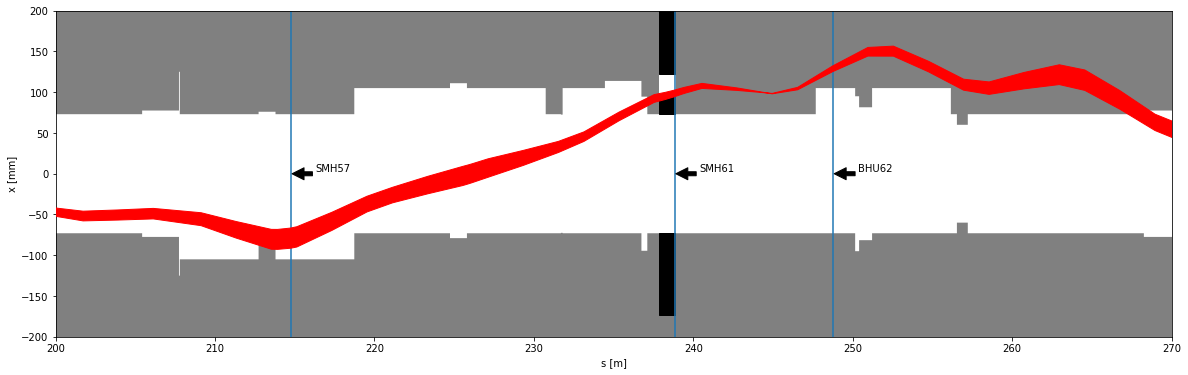
\includegraphics[width=1.0\textwidth]{02_Simulation/images/beam_envelope.png}
\caption{Beam envelope through SMH57, SMH61 and at the entrance of MU62.}
\label{fig:beam_envelope}
\end{figure}


\begin{table}[htbp]
\centering
\caption{Initial condition upstream of the MU62 magnet}
\label{tab:twiss_parameters}
\begin{tabular}{|c|c|c|c|c|c|c|c|}
\hline
$\beta_{x}$ [m] & $\beta_{y}$ [m] & $\alpha_{x}$ & $\alpha_{y}$ & $D_{x}$ [m] & $D_{y}$ [m] & $D^{'}_{x}$[mrad] & $D^{'}_{y}$[mrad] \\
\hline
7.48 & 26.14 & 0.0021 & 0.0591 & 1.428 & 0.0 & -0.021 & 0.0 \\
\hline
\end{tabular}
\end{table}


The MFC model was added to the default F61D transfer line sequence in MAD-X, see Fig. \ref{fig:f61d_with_stray}. The F61D with stray field line \href{https://gitlab.cern.ch/eljohnso/acc-models-tls-eliott-fork/-/blob/c6cbcafacca274000d2bfc501f39cf711375de90/ps_extraction/east-fast-extraction/f61d_with_stray/F61D_with_stray.ipynb}{script} has the stray field element of the MU62 magnet decomposed into multipole and can be found at \href{https://gitlab.cern.ch/eljohnso/acc-models-tls-eliott-fork/-/blob/c6cbcafacca274000d2bfc501f39cf711375de90/ps_extraction/east-fast-extraction/f61d_with_stray/strayMU62.ele}{strayMU62.ele} and \href{https://gitlab.cern.ch/eljohnso/acc-models-tls-eliott-fork/-/blob/c6cbcafacca274000d2bfc501f39cf711375de90/ps_extraction/east-fast-extraction/f61d_with_stray/strayMU62.seq}{strayMU62.seq}. Using the initial conditions upstream of MU62 and the PS lattice, a Twiss computation was run to compare the initial parameters between the simulation and measurements. It is important to note that the initial conditions derived from the PS lattice are upstream of the MU62 magnet, whereas the initial conditions from empirical measurements are taken after the MU62 magnet and before the Q74L magnet. For details on how the initial parameters were determined through measurement, see Section \ref{initial beam parameters empirical}.

\begin{figure}[H]
\centering
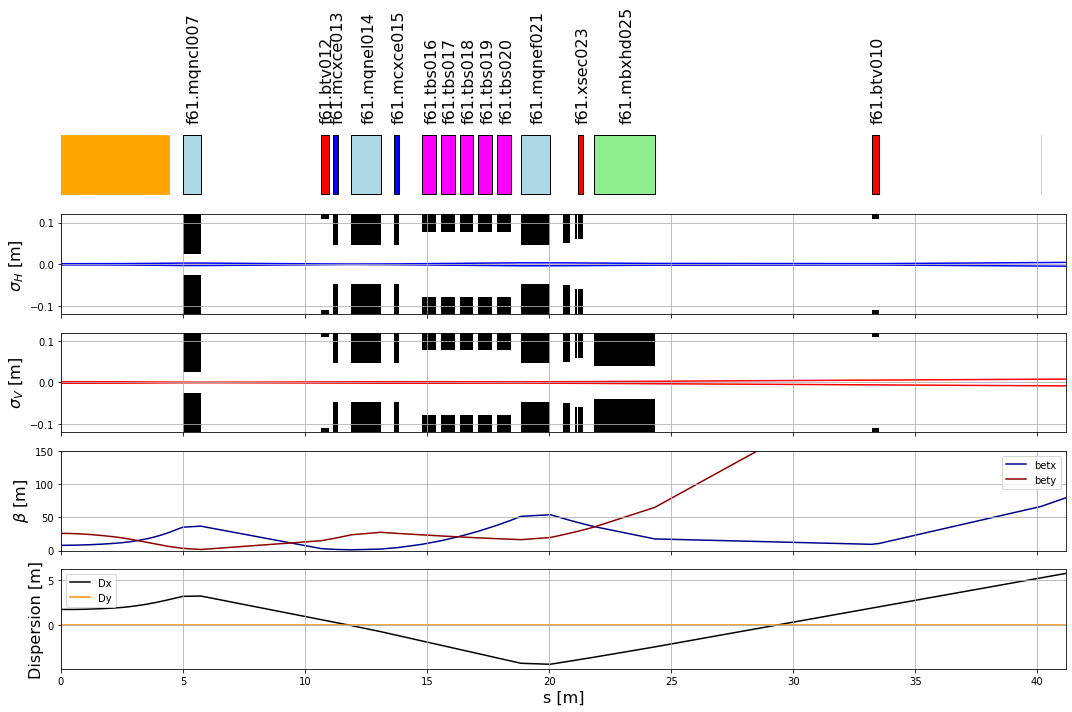
\includegraphics[width=1.0\textwidth]{02_Simulation/images/F61D_with_stray.png}
\caption{F61D with stray field multipole of MU62. The orange rectangle in the synoptic is a representation the multipole component of the stray field.}
\label{fig:f61d_with_stray}
\end{figure}


\begin{table}[htbp]
\centering
\caption{Comparison of Simulated and Measured Twiss Parameters after the MU62 stray fields, upstream of Q74L.}
\label{tab:twiss_comparison}
\begin{tabular}{|c|c|c|c|c|c|c|c|c|}
\hline
& $\beta_{x}$ [m] & $\beta_{y}$ [m] & $\alpha_{x}$ & $\alpha_{y}$ & $D_{x}$ [m] & $D_{y}$ [m] & $D^{'}_{x}$ [mrad] & $D^{'}_{y}$ [mrad] \\
\hline
\textbf{Simulated} & 35 & 3.4 & -7.4 & 2.1 & 3.2 & 0 & 0.63 & 0 \\
\hline
\textbf{Measured} & 154 & 5.2 & -37 & 0.25 & 0.13 & 0 & 0.02 & 0 \\
\hline
\end{tabular}
\end{table}

The comparison of the simulated and measured Twiss parameters after the MU62 stray fields reveals significant discrepancies. The simulated values for $\beta_{x}$, $\alpha_{x}$, and $D_{x}$ show considerable deviations from the measured data, with the simulated $\beta_{x}$ and $\alpha_{x}$ being notably lower than the measured values. These differences suggest that the simulation model does not accurately capture the conditions observed in the empirical measurements. Further section will try to identify the underlying causes of these discrepancies and to improve the accuracy of the simulation model by adding additional stray field maps to achieve better alignment between simulation and measurement.


\subsection{Stitched model}

The slow extraction process cannot be adequately described using Twiss parameters alone; it requires detailed tracking. Particles at the edge of the septum blade make three turns and are extracted on the fourth, while those outside the septum blade are extracted in the current turn.

The \href{https://gitlab.cern.ch/eljohnso/acc-models-tls-eliott-fork/-/blob/EliottBranch/ps_extraction/east-fast-extraction/stitched_slow_extraction_east_PTC_single_turn.ipynb}{script} tracks the pycollimate distribution in the PS, save the distribution at the entrance of MU62, remove the mean x and xp and then tracks it in the F61D line. This simulation also include the MFC of MU63.

\begin{table}[htbp]
\centering
\caption{Initial condition upstream of the MU62 magnet}
\label{tab:twiss_parameters}
\begin{tabular}{|c|c|c|c|c|c|}
\hline
$\beta_{x}$ [m] & $\beta_{y}$ [m] & $\alpha_{x}$ & $\alpha_{y}$ & $\epsilon_x$ [m] & $\epsilon_y$ [m] \\
\hline
167.32 & 1.21 & 21.61 & 0.33 & $1.78 \times 10^{-7}$ & $3.8 \times 10^{-8}$ \\
\hline
\end{tabular}
\end{table}

\begin{figure}[H]
\centering
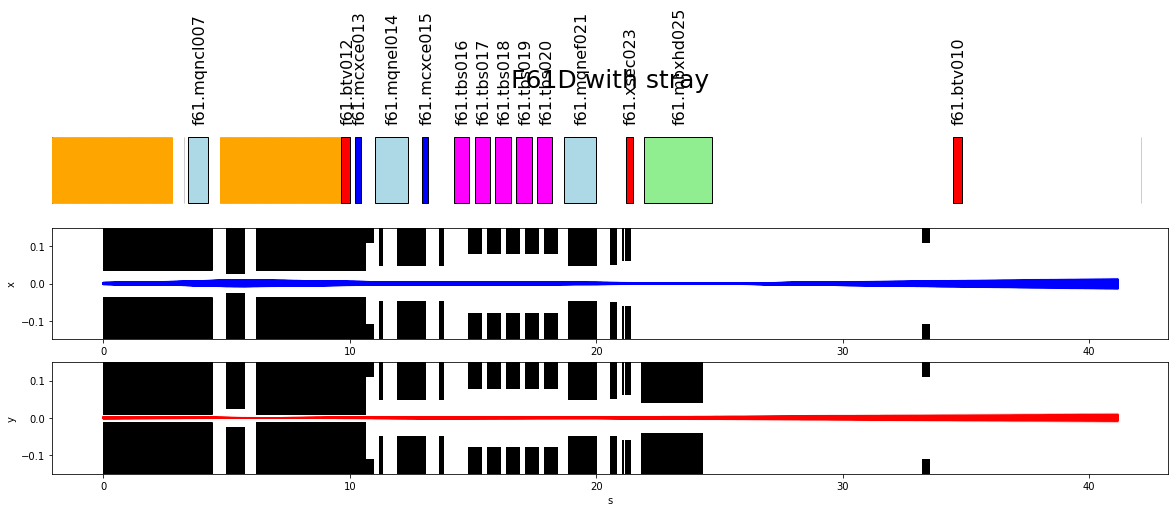
\includegraphics[width=1.0\textwidth]{02_Simulation/images/PTC_stray_field.png}
\caption{Stitched model PTC tracking.}
\label{fig:stitched_PTC}
\end{figure}

\subsection{Repository with the Full Stitching from the PS Ring to the East Dump}

The repository containing all necessary scripts is available at \href{https://gitlab.cern.ch/eljohnso/stray-fields}{stray-fields}.

\begin{itemize}
    \item \textbf{Step one:} Create the distribution upstream of SEH23 using pycollimate. This is done using this \href{https://gitlab.cern.ch/eljohnso/stray-fields/-/blob/master/pycollimate.ipynb}{script}, which generates the \texttt{distribution\_at\_seh23.pkl} file.
    \item \textbf{Step two:} Run \href{https://gitlab.cern.ch/eljohnso/stray-fields/-/blob/master/ps_ring.ipynb?ref_type=heads}{ps ring}, which tracks the particle distribution in the PS ring and outputs the distribution before entering MU62.
    \item \textbf{Step three:} Run \href{https://gitlab.cern.ch/eljohnso/stray-fields/-/blob/master/f61d_tracking.ipynb?ref_type=heads}{f61d tracking}, which takes the distribution entering MU62 and tracks it in the F61D line.
\end{itemize}

\begin{figure}[H]
\centering
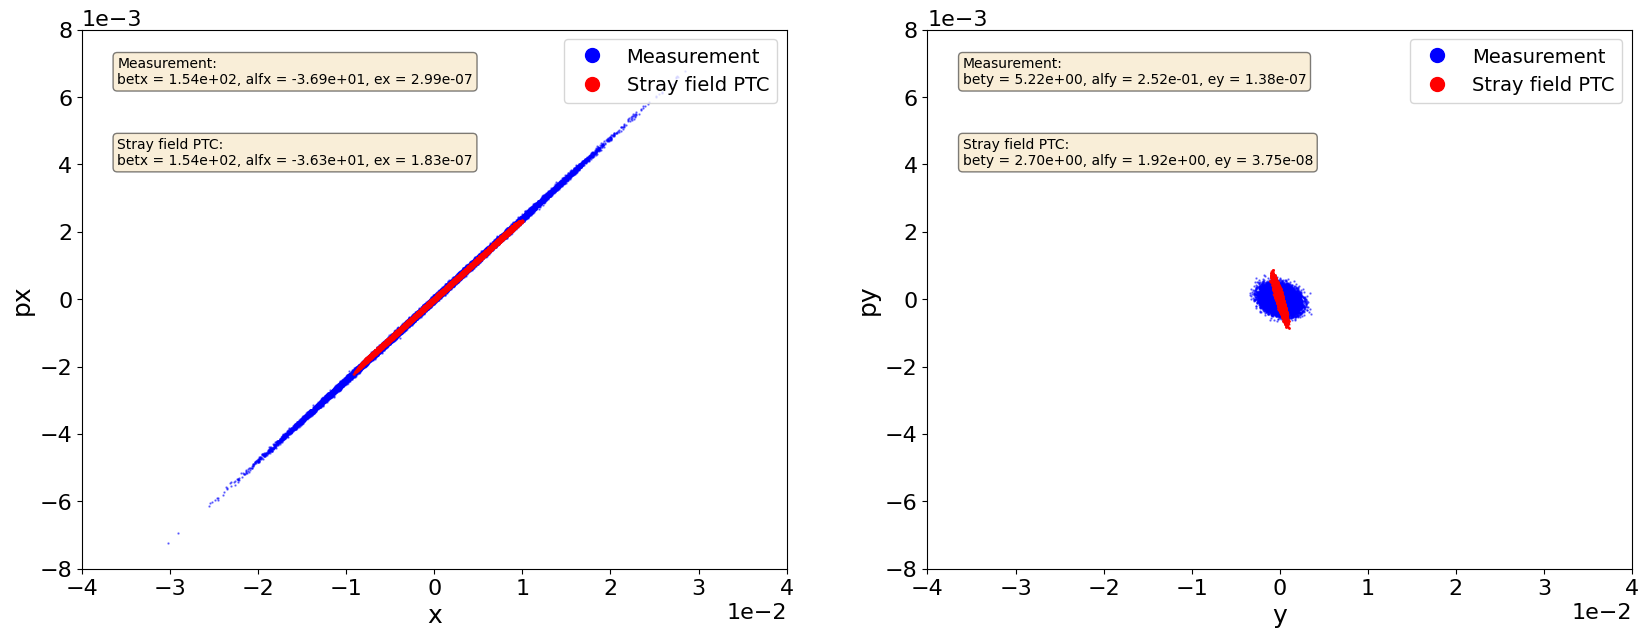
\includegraphics[width=1.0\textwidth]{02_Simulation/images/full_stitching_PTC.png}
\caption{Full stitched model PTC tracking and comparison with measurements.}
\label{fig:full_stitched_PTC}
\end{figure}

It is important to note that the distribution obtained from tracking is non-Gaussian, which may result in discrepancies when computing the Twiss parameters.

\begin{figure}[H]
\centering
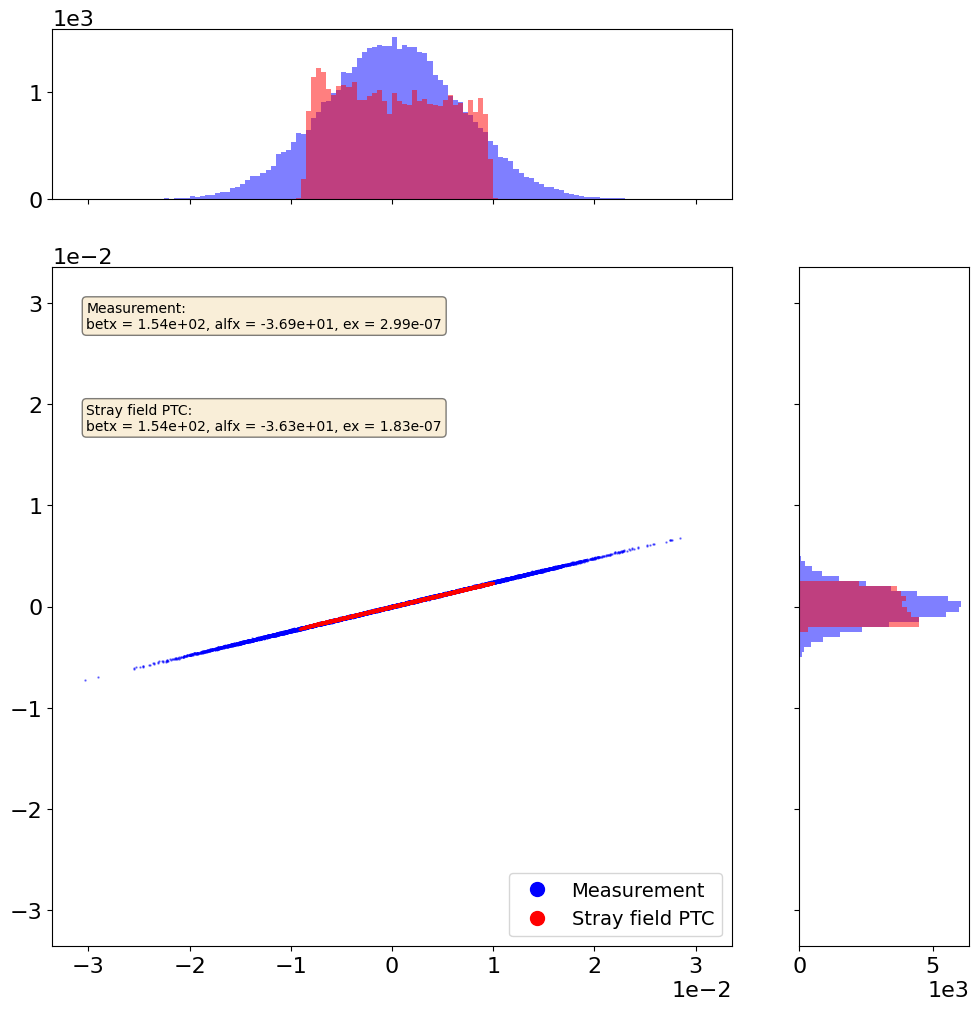
\includegraphics[width=1.0\textwidth]{02_Simulation/images/non_gaussian.png}
\caption{The distributions are non-Gaussian.}
\label{fig:non_gaussian}
\end{figure}

Table \ref{tab:twiss_parameters} compares the initial parameters found upstream of MU62 using the full stitched model or the empirical measurement.

\begin{table}[htbp]
\centering
\caption{Initial condition upstream of the MU62 magnet}
\label{tab:twiss_parameters}
\begin{tabular}{|c|c|c|c|c|c|c|}
\hline
Label & $\beta_{x}$ [m] & $\beta_{y}$ [m] & $\alpha_{x}$ & $\alpha_{y}$ & $\epsilon_x$ [m] & $\epsilon_y$ [m] \\
\hline
Stray Field PTC & $154$ & $2.70$ & $-36.3$ & $1.92$ & $1.83 \times 10^{-7}$ & $3.75 \times 10^{-8}$ \\
\hline
Measurement & $154$ & $5.22$ & $-36.9$ & $0.252$ & $2.99 \times 10^{-7}$ & $1.38 \times 10^{-7}$ \\
\hline
\end{tabular}
\end{table}

Instead of displaying the particle distribution, it may be more informative to examine the differences in the ellipses, as shown in Fig. \ref{fig:ellipses}.

\begin{figure}[H]
\centering
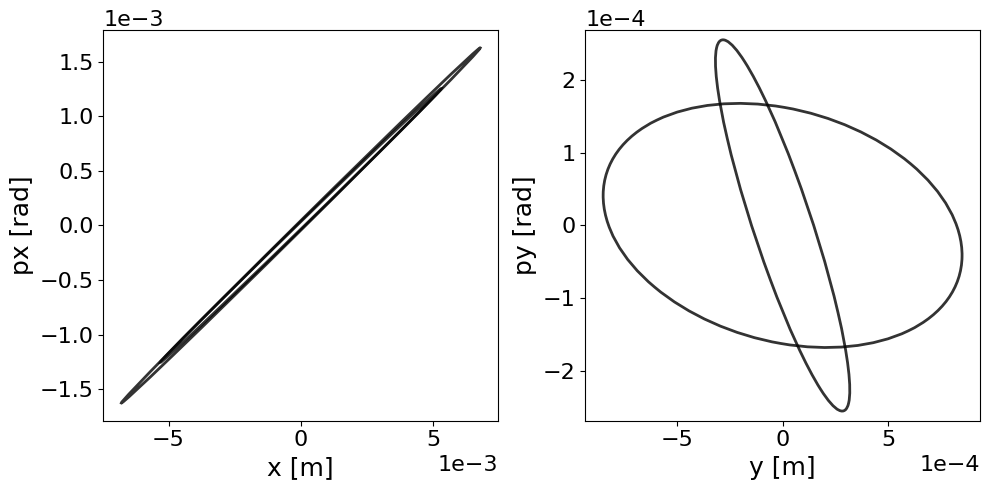
\includegraphics[width=1.0\textwidth]{02_Simulation/images/ellipses.png}
\caption{Comparison between the ellipses produced by the Twiss parameters of the simulation and the tracking.}
\label{fig:ellipses}
\end{figure}

Additionally, we can examine the evolution of the Twiss parameters along the line, as shown in Fig. \ref{fig:twiss_params}.

\begin{figure}[H]
\centering
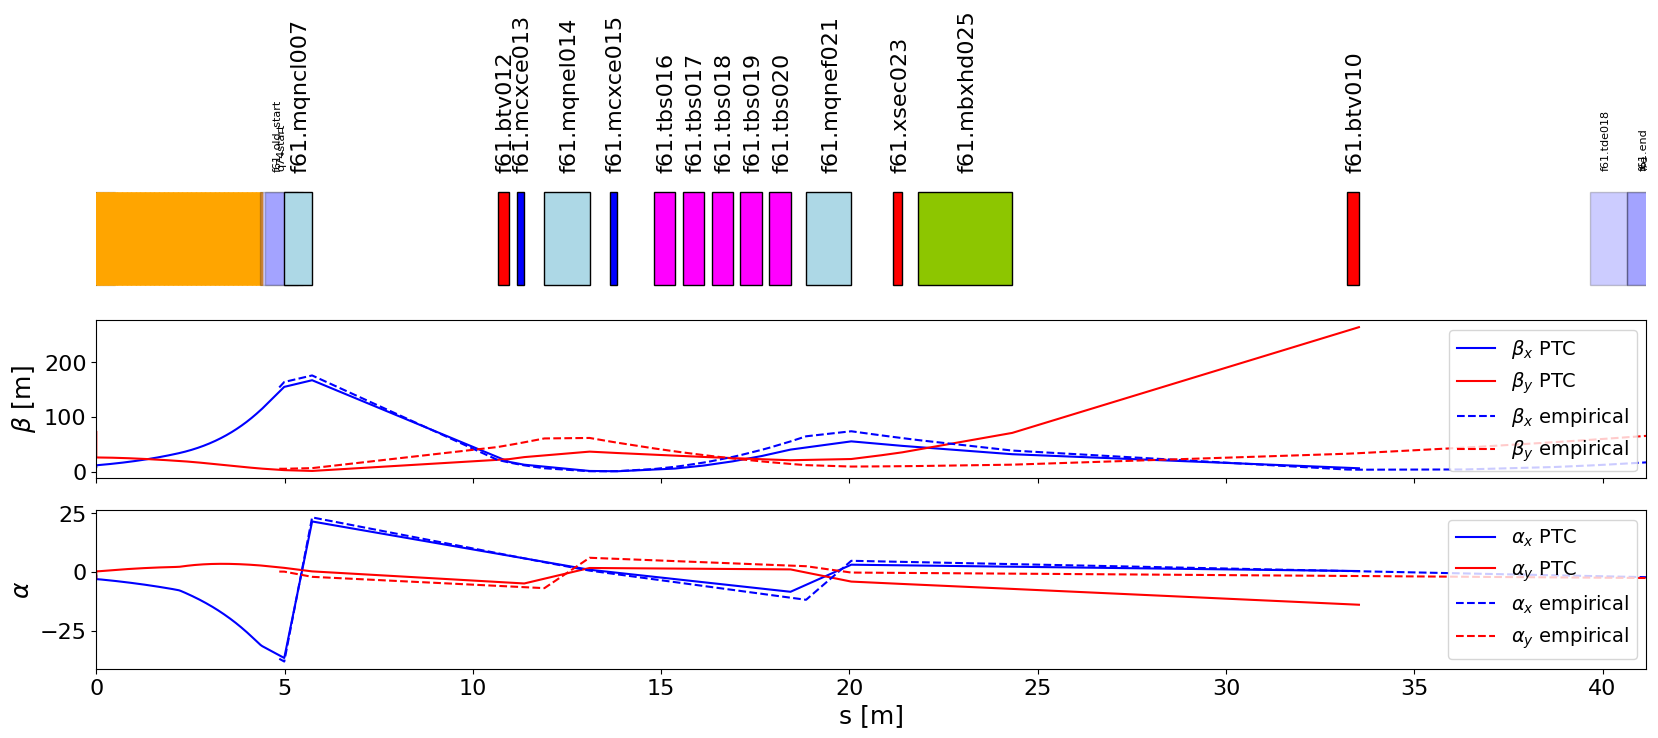
\includegraphics[width=1.0\textwidth]{02_Simulation/images/twiss_parameters_comparison.png}
\caption{Comparison between the Twiss parameters along the line of the simulation and the empirical measurement.}
\label{fig:twiss_params}
\end{figure}

From the previous plots, it is evident that the horizontal model performs well, whereas the description of the vertical plane is less accurate. To investigate the impact on the particle distribution, I replaced the horizontal MFC model with a vertical MFC model, calculating $B_{x}$ as follows:
\[
B_{x} = \begin{bmatrix}  
x_{\text{center}} \\  
y_{\text{offset}} \\
z_{\text{center}} 
\end{bmatrix}
\]

Including the coupling terms (which should be small) $B_{y}(y)$, $B_{x}(x)$, and $\frac{\partial^{k} B_{i}}{\partial x_{j}^{k}}$, we observe no significant difference between using the MCP model for $\frac{\partial B_{y}}{\partial x}$ or $\frac{\partial B_{x}}{\partial y}$. Both yield similar results in the horizontal and vertical planes. This is illustrated in Fig. \ref{fig:coupling_terms}, which shows that the second-order terms are identical. Thus, it appears that the initial distribution in the PS ring for the vertical plane may be incorrect.

\begin{figure}[H]
\centering
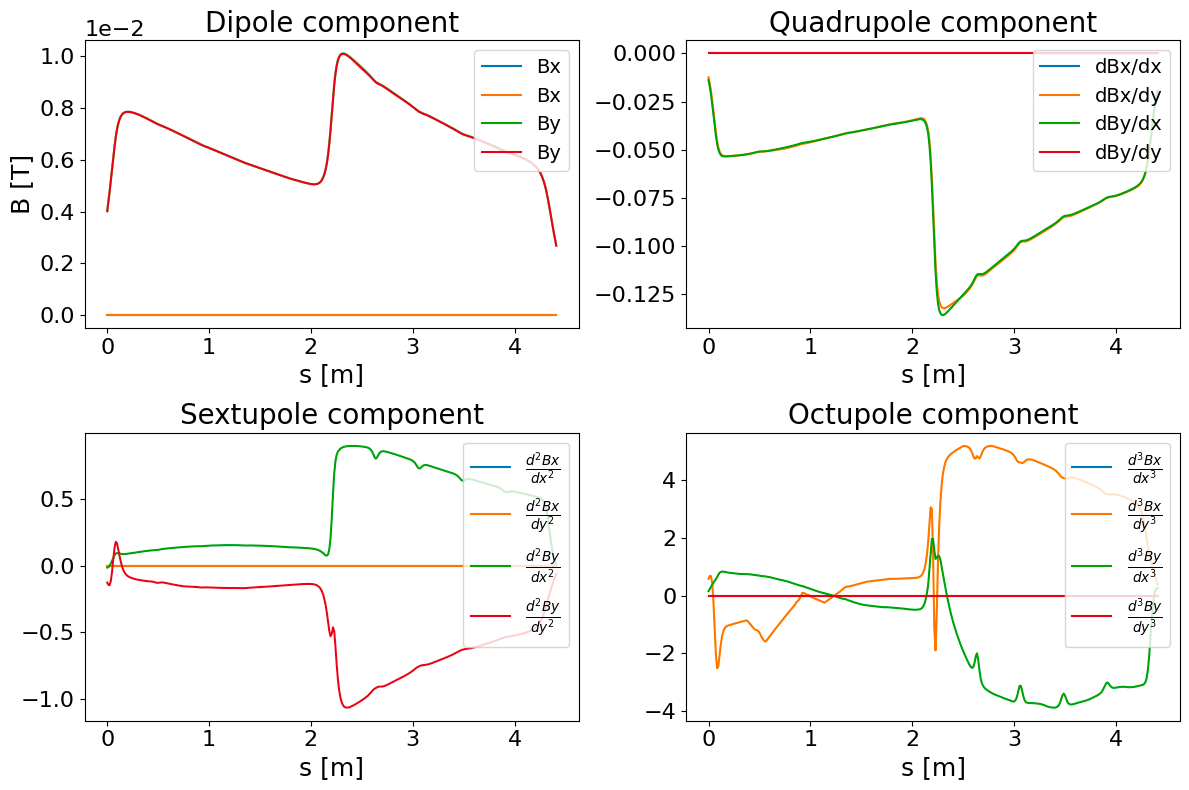
\includegraphics[width=1.0\textwidth]{02_Simulation/images/coupling_terms.png}
\caption{Coupling terms.}
\label{fig:coupling_terms}
\end{figure}

Figure \ref{fig:comparison_sim_meas} shows the difference between the beam size observed at the BTV of the East Dump through simulation and beam size measurement. We observe excellent agreement in the horizontal plane but a mismatch in the vertical plane.

\begin{figure}[H]
\centering
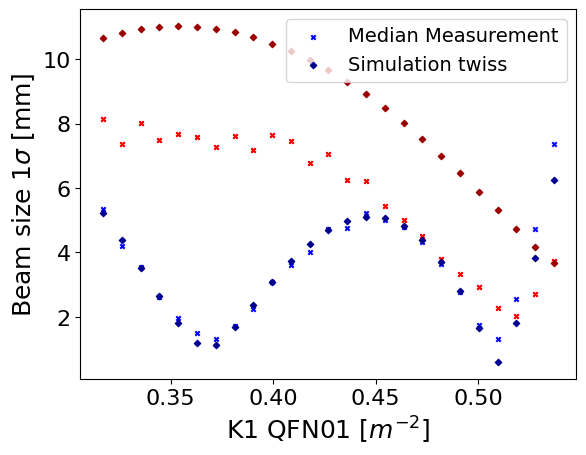
\includegraphics[width=0.7\textwidth]{02_Simulation/images/comparison_sim_meas.png}
\caption{Comparison between the simulated and measured beam size at the BTV of the East Dump.}
\label{fig:comparison_sim_meas}
\end{figure}




\subsection{MU63}

To fix the mismatch in the vertical plane, the MU63's stray fields were computed by tracking the particle reference trajectory and extracting the MFC, see Fig. \ref{fig:track_mu63} and \ref{fig:mfc_mu63}.

\begin{figure}[H]
\centering
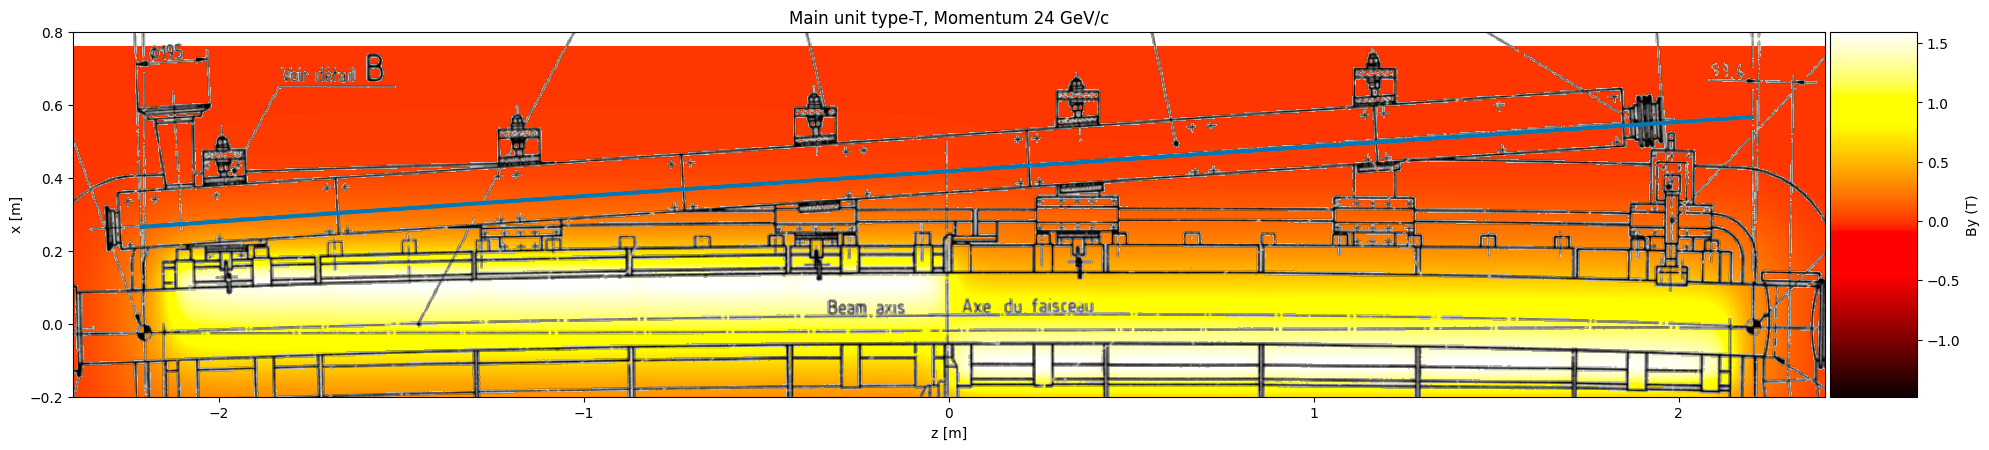
\includegraphics[width=1.0\textwidth]{02_Simulation/images/track_mu63.png}
\caption{Particle tracking through MU63.}
\label{fig:track_mu63}
\end{figure}

\begin{figure}[H]
\centering
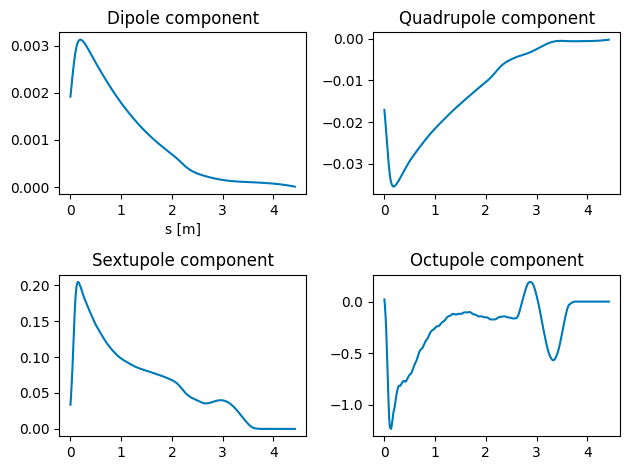
\includegraphics[width=1.0\textwidth]{02_Simulation/images/mfc_mu63.png}
\caption{MFC model of MU63.}
\label{fig:mfc_mu63}
\end{figure}

However, including the full multipole components of the MU63 is incorrect since the MU63 has shims that straighten the B-field component, significantly reducing the quadrupolar component. Therefore, only the dipole component was retained, which, as expected, does not alter the optics.
\\
\\
From this, it appears that the optics in the horizontal plane are correct but mismatched in the vertical plane. This suggests the need to add a quadrupole component at a very low $\beta_{x}$ location upstream of the F61D line. Possibly, in MU61, where the excursion is already quite large, there might be a quadrupole component. Consequently, the MU61 quadrupole component was optimized by slightly adjusting the values and minimizing the difference between measurement and simulation using Pybobyqa. The results were slightly better but not significantly improved.
\\
\\
Subsequently, the four quadrupole components of MU60 and MU61, the two main units before extraction, were optimized. In these units, the transverse excursion is already considerable, and the quadrupole component is not aligned with the reference orbit. Each dipole has two quadrupole components, resulting in four parameters to optimize.
\\
\\
The actual quadrupole components at the excursion were simulated using the opera model, which provided the values shown in Table \ref{tab:quadrupole_components} and Fig. \ref{fig:comparison_four_compo}.

\begin{table}[htbp]
\centering
\caption{Simulated quadrupole components at the excursion using the opera model}
\label{tab:quadrupole_components}
\begin{tabular}{|l|c|}
\hline
Component & Value \\
\hline
pr.bht61.f & 0.02723 \\
pr.bht61.d & -0.05518 \\
pr.bhu60.f & 0.04969 \\
pr.bhu60.d & -0.05831 \\
\hline
\end{tabular}
\end{table}

\begin{figure}[H]
\centering
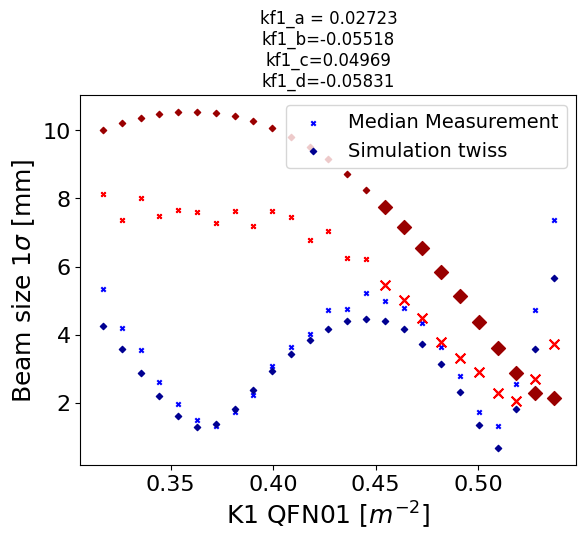
\includegraphics[width=0.7\textwidth]{02_Simulation/images/comparison_sim_meas_four_compo.png}
\caption{Comparison four components.}
\label{fig:comparison_four_compo}
\end{figure}

Running the optimizer algorithm, it converges on different quadrupole components with a better match between beam size and simulation.

\begin{figure}[H]
\centering
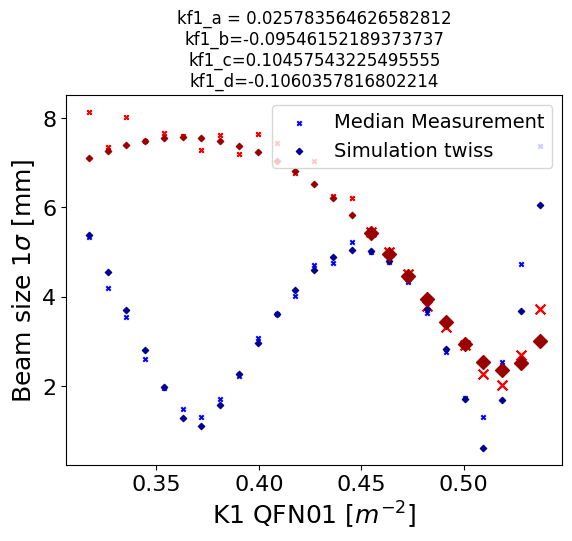
\includegraphics[width=0.7\textwidth]{02_Simulation/images/comparison_sim_meas_bobyqa.png}
\caption{Comparison of beam size and simulation using pybobyqa.}
\label{fig:comparison_bobyqa}
\end{figure}

\subsection{Replacing MU60 and MU61 with stray fields}

From previous notes, it seems replacing only MU62 matched well the measurement in the horizontal plane but not in the vertical plane.

Adding MU63 doesn't help correcting the mismatch in the vertical plane because it's in a region of high $\beta_{x}$ which would change the optics in that plane and additionally it is shimmed so I don't think there is much quadrupolar effect, thus I've added only the dipole component of this magnet.

I've then thought about the large excursion in the two preceding main units, MU60 and MU61 and tried to optimise on the four quadrupole component that are in the PS lattice file.

I found some solution that match the measurement pretty well but they are very different.

\begin{table}[ht]
    \centering
    \caption{Twiss Parameters for MU60 and MU61}
    \begin{tabular}{l c c c c}
        \hline
        & \textbf{MU60 d} & \textbf{MU60 f} & \textbf{MU61 f} & \textbf{MU61 d} \\
        \hline
        Row 1 & -0.1 & 0.1 & 0.0046 & -0.0862 \\
        Row 2 & -0.094 & 0.1026 & -0.0247 & -0.0231 \\
        Row 3 & -0.106 & 0.1045 & 0.0258 & -0.0955 \\
        \hline
    \end{tabular}
    \label{tab:twiss_parameters_mu60_mu61}
\end{table}



If we compute the quadrupole component of MU60 and MU61 along the trajectory that ejects the beam, we see that the quadrupolar component can not be approximated by a single number.

\begin{figure}[H]
\centering
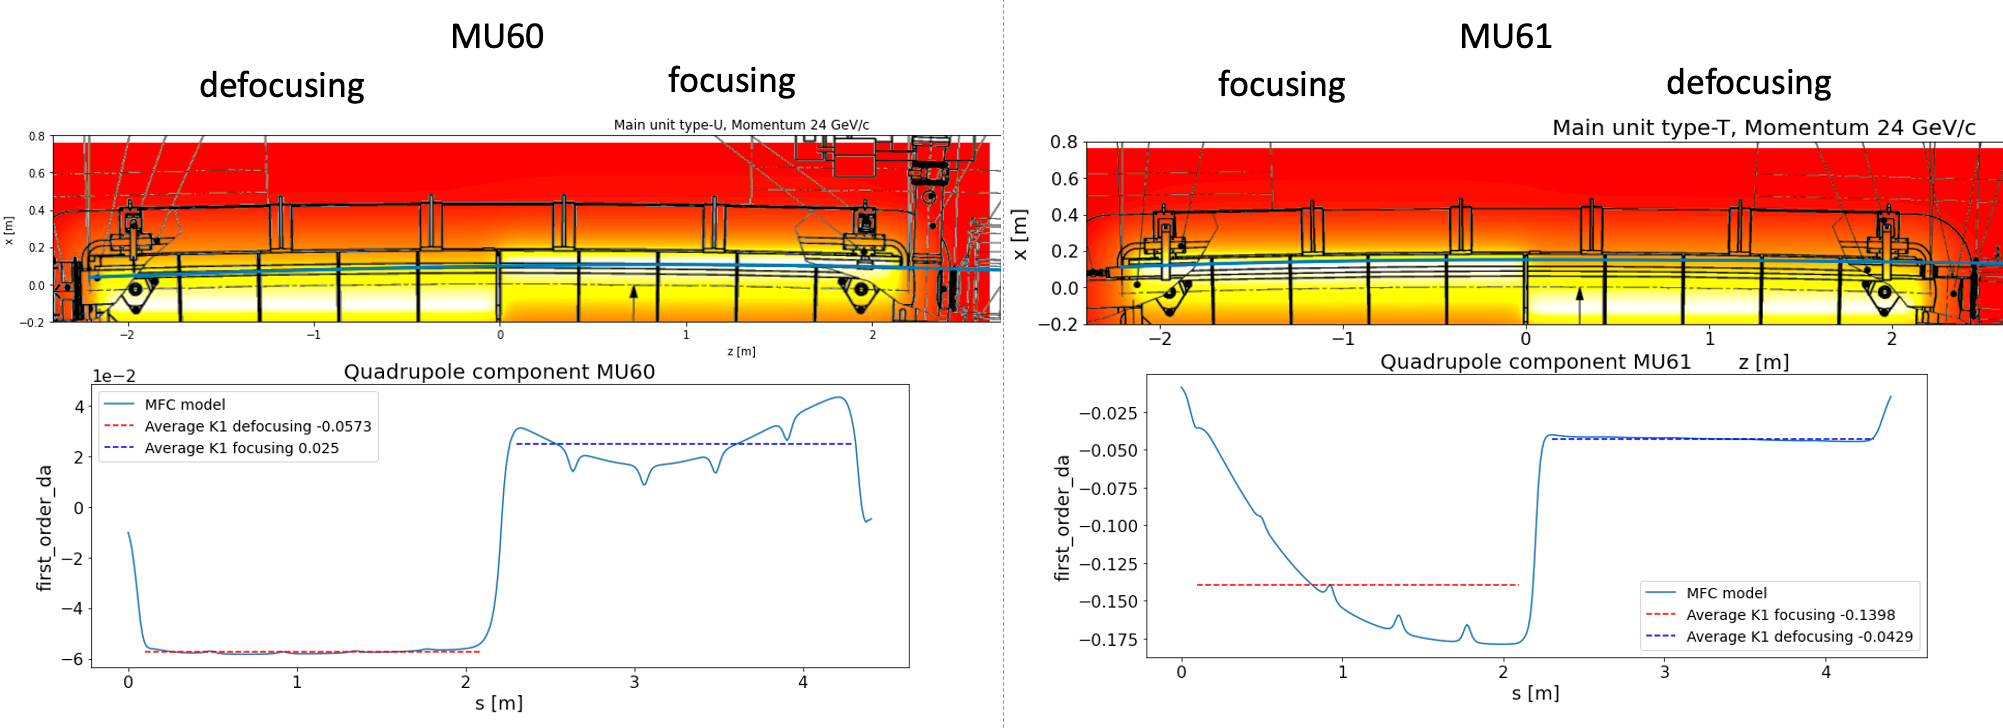
\includegraphics[width=1.0\textwidth]{02_Simulation/images/mu60_mu61_quad_comp.png}
\caption{MU60 and MU61 quadrupole components.}
\label{fig:mu60_mu61_q_comp}
\end{figure}

If we compute an average quadrupole component in these regions and use them in the simulation it does not give good results, see Fig. \ref{fig:replace_with_average}. With these numbers the mismatch is quite high. I then think we need to replace with the full MFC model for both magnet and see how it behave.

\begin{figure}[H]
\centering
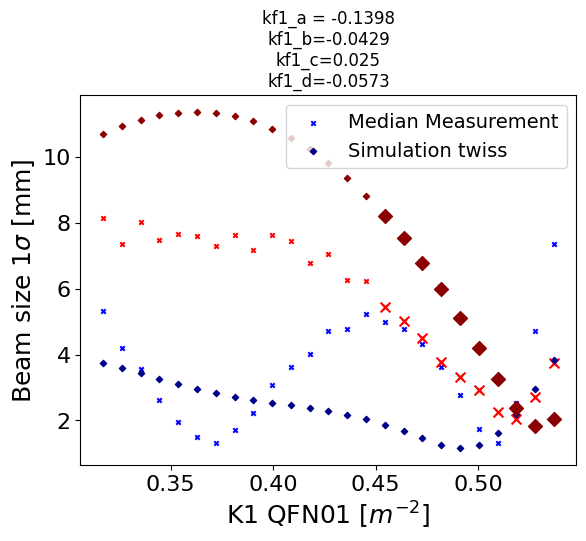
\includegraphics[width=0.7\textwidth]{02_Simulation/images/Replace MU60 and MU61 with stray field-2.png}
\caption{Replace MU60 and MU61 quadrupole components with average components.}
\label{fig:replace_with_average}
\end{figure}

\subsection{Adding the full stray fields of MU60 and MU61}

To add the stray field MCP model of MU60 and MU61 in the PS lattice, the PR.MP60 and PR.MP61 elements where removed from the lattice and the MCP where inserted instead. Figure \ref{fig:mcp_mu60_mu61} shows the results in this configuration.

\begin{figure}[H]
\centering
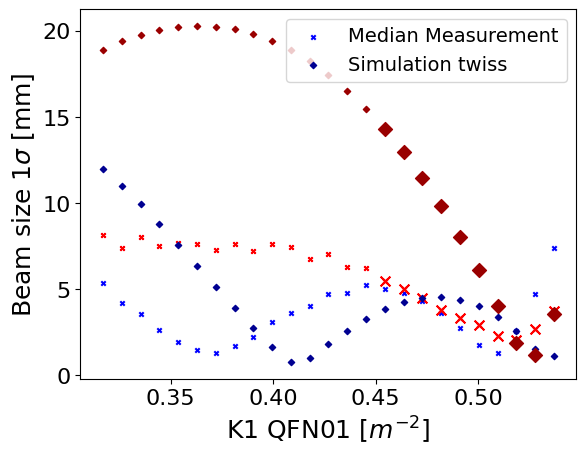
\includegraphics[width=0.7\textwidth]{02_Simulation/images/mcp_mu60_mu61.png}
\caption{Replace MU60 and MU61 with full stray field components.}
\label{fig:mcp_mu60_mu61}
\end{figure}

One thing I don't understand is the excursion with stray MU60 and MU61 is larger then just a drift, see Fig. \ref{excursion_m60_mu61_mcp}. 

I think it's because we have an large x-excursion which create a dipole moment from the quadrupole component. I should try to set x to zero.

\begin{figure}[H]
\centering
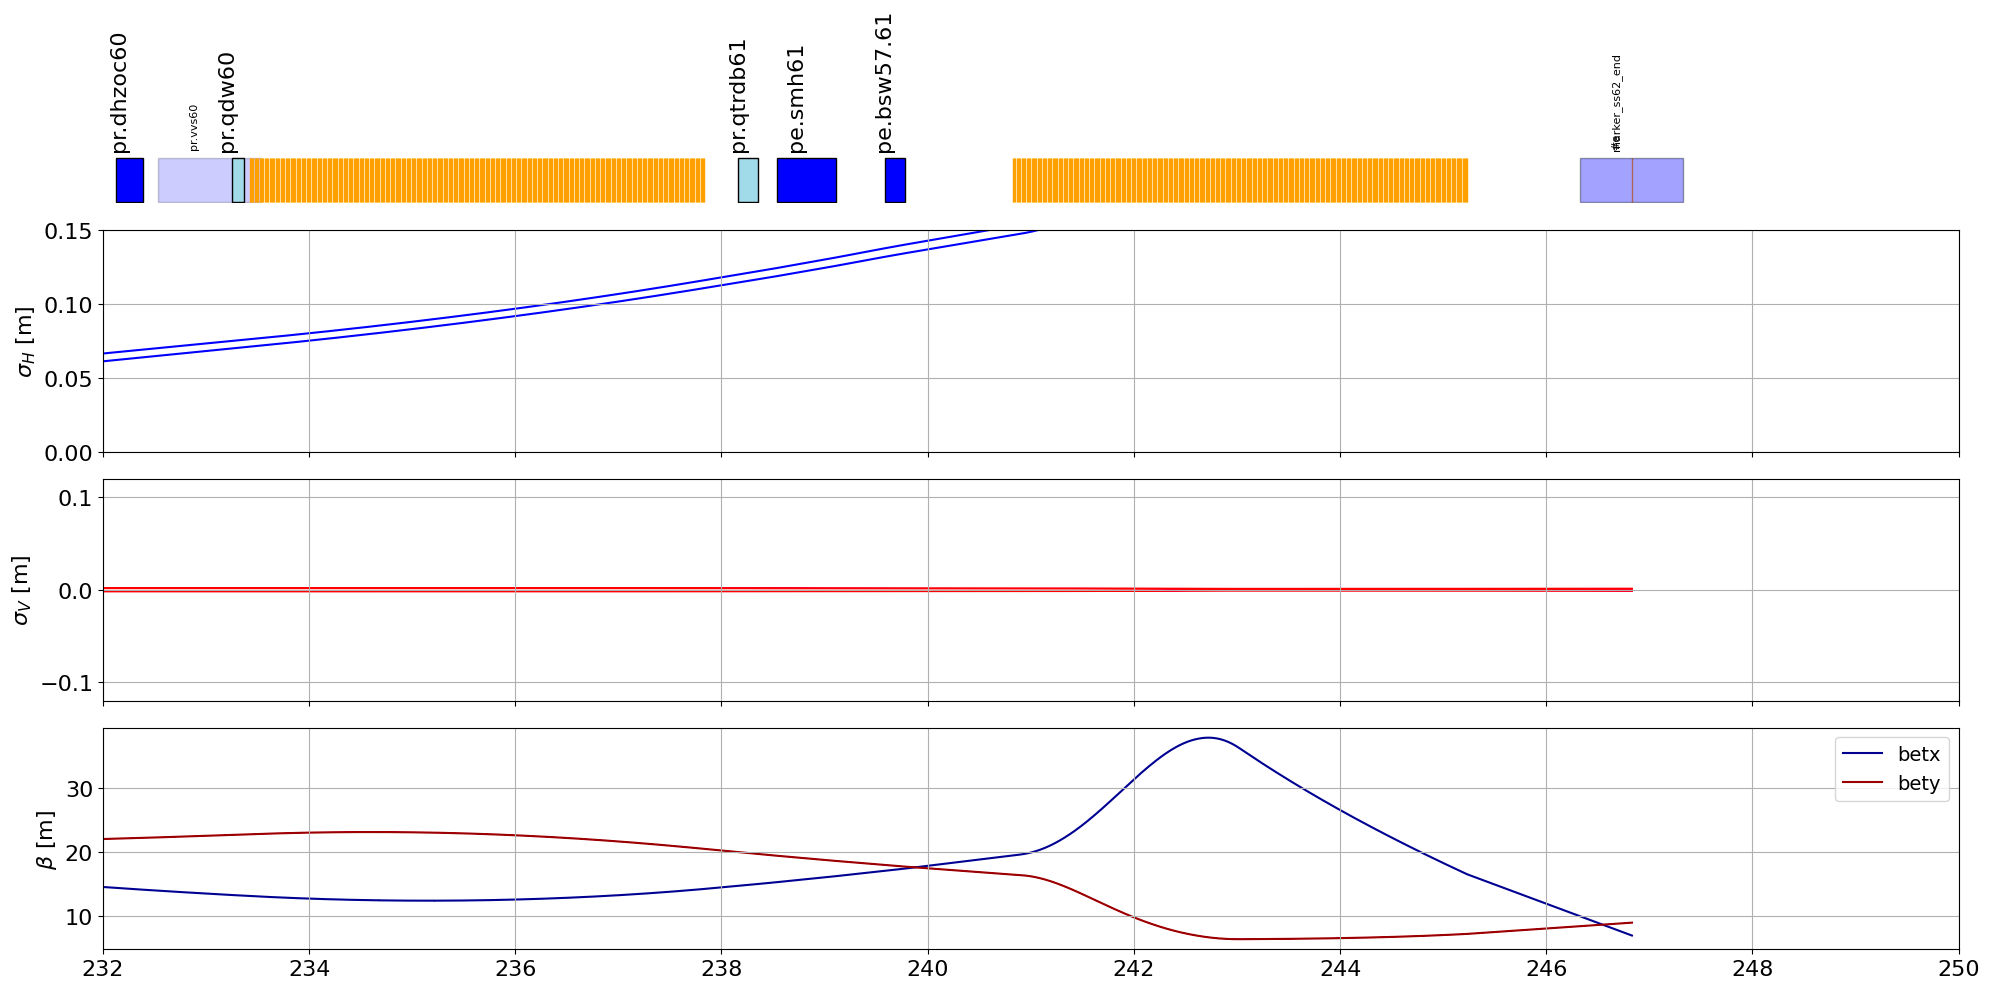
\includegraphics[width=0.7\textwidth]{02_Simulation/images/excursion_mu60_mu61_mcp.png}
\caption{Excusrion MU60 and MU61 with full stray field components.}
\label{fig:excursion_m60_mu61_mcp}
\end{figure}

Additional issues is that the MCP in these magnets is very dependant on the trajectory of the track of the reference particle that is launched to create the MCP map. Launching with slight offsets in angle and position will dramatically change the quadrupole component profile.

\subsection{Simulation of Transfer Matrix Using Tracking at Injection}

The following subsection describes the methodology and findings from a simulation study aimed at constructing a transfer matrix for the injection process in the Proton Synchrotron (PS) using tracking techniques. The primary objective is to evaluate the response of injected particles to various initial offsets and to compare the results with existing models.

A comprehensive simulation was performed using the  \href{https://gitlab.cern.ch/eljohnso/acc-models-tls-eliott-fork/-/blob/EliottBranch/ps_injection/kick_response_injection_tracking/kick_response_BTP_injection_loop_transfer_matrix.ipynb}{kick response BTP injection loop transfer matrix} notebook. This notebook tracks particles injected into the PS at different initial offsets in the transverse and longitudinal planes. Specifically, four types of initial offsets were used: horizontal position (\(x_{in}\)), horizontal angle (\(p_{x,in}\)), vertical position (\(y_{in}\)), and vertical angle (\(p_{y,in}\)). The resulting offsets at the output (\(x_{out}\), \(p_{x,out}\), \(y_{out}\), \(p_{y,out}\)) were recorded to construct the transfer matrix.

\begin{figure}[H]
\centering
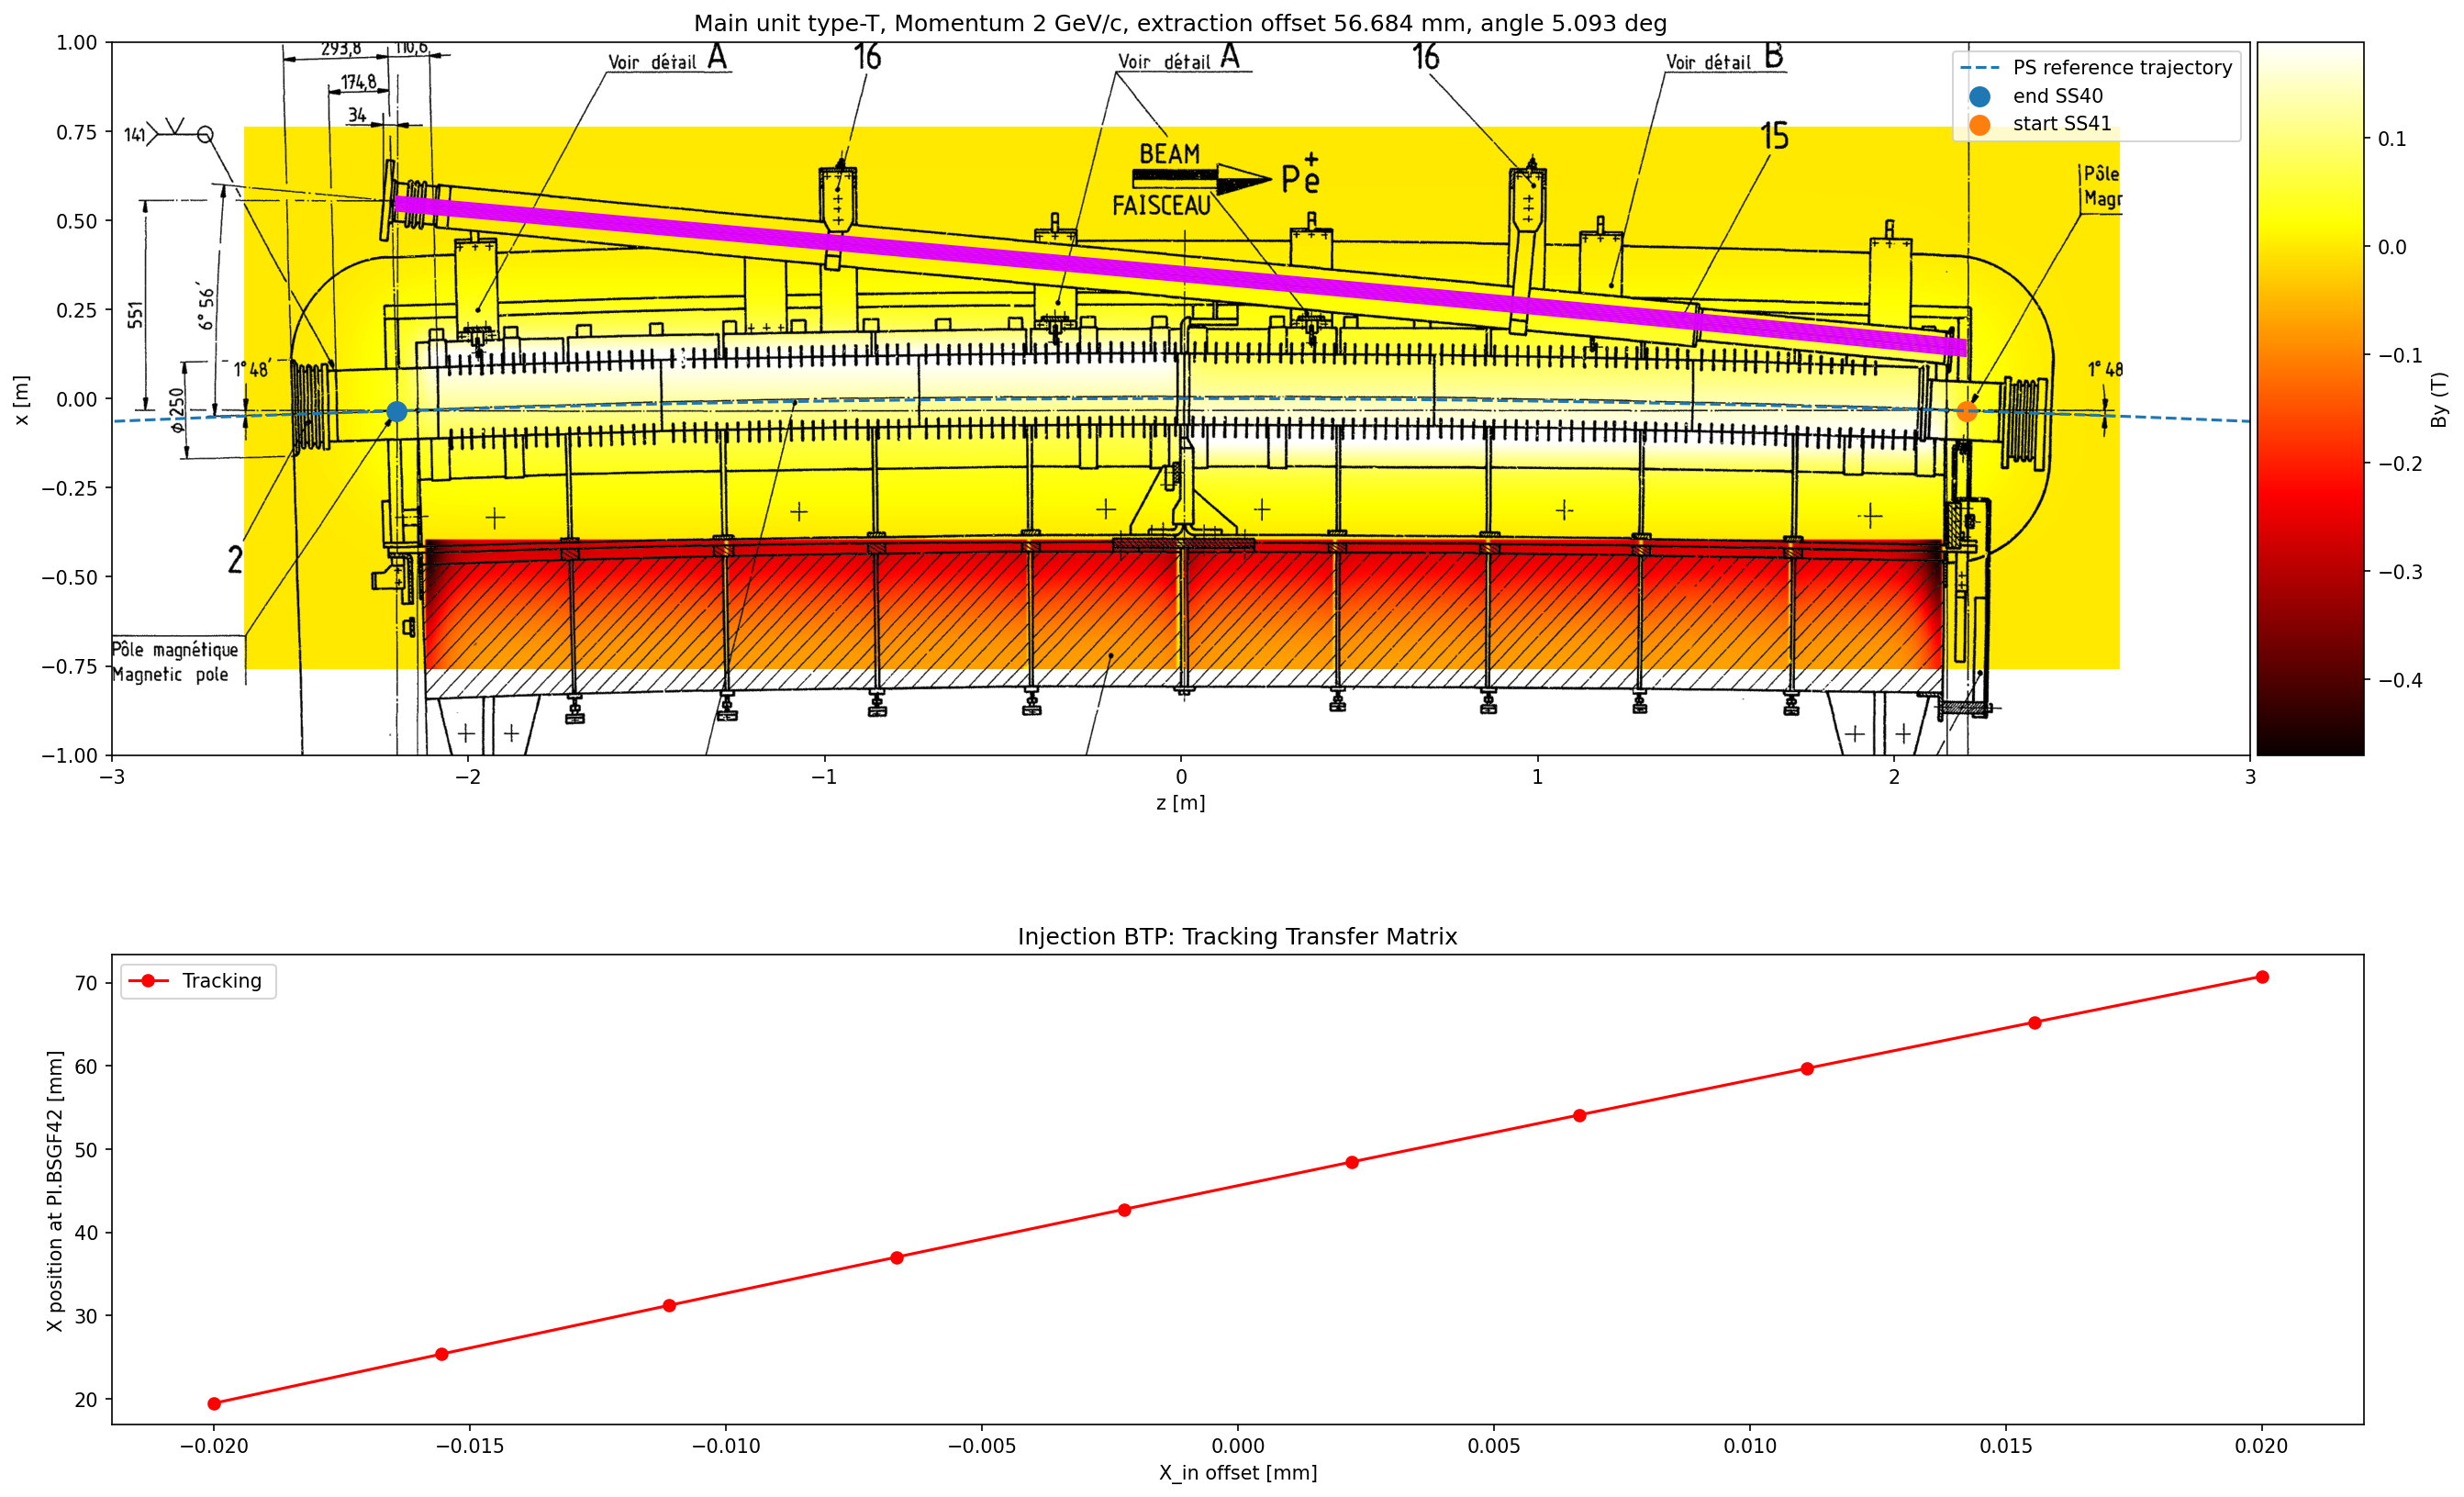
\includegraphics[width=1.0\textwidth]{02_Simulation/images/injection_transfer_matrix_1.png}
\caption{Building a transfer matrix through tracking.}
\label{fig:transfer_matrix_1}
\end{figure}

\begin{figure}[H]
\centering
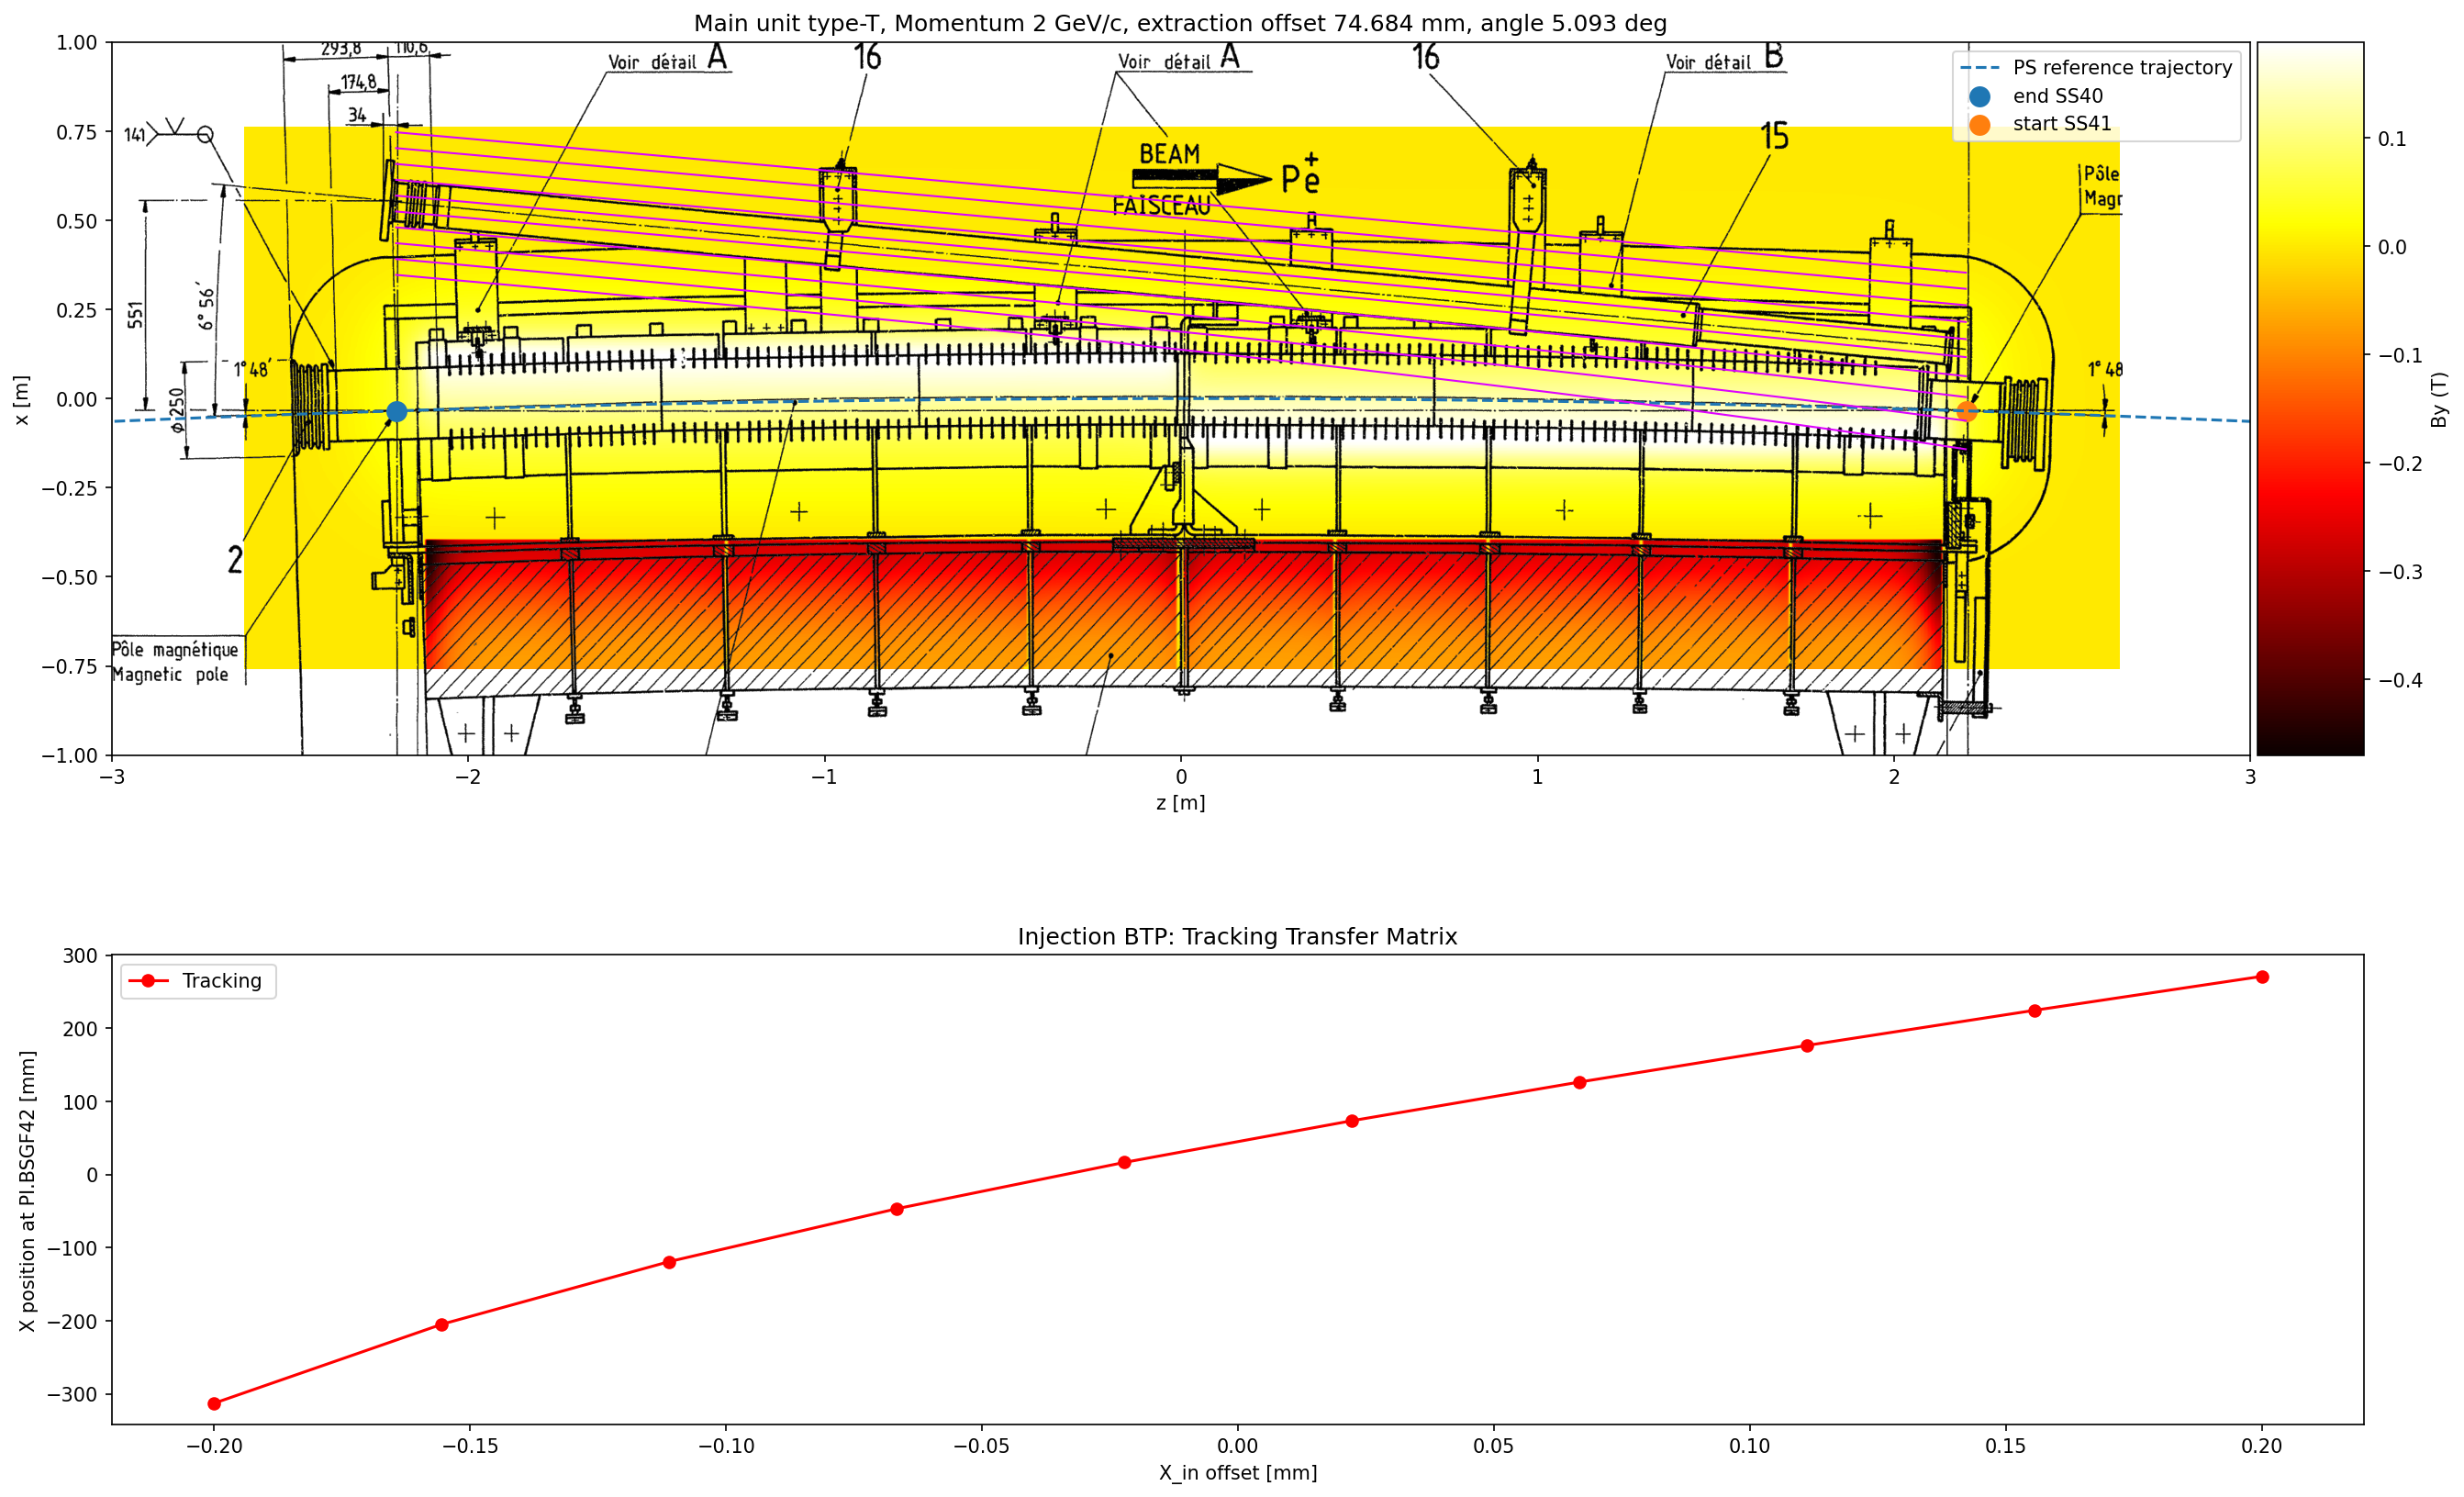
\includegraphics[width=1.0\textwidth]{02_Simulation/images/injection_transfer_matrix_2.png}
\caption{Wide scan of the position offset to see if the response is non-linear.}
\label{fig:transfer_matrix_2}
\end{figure}


The simulation can cover a wide range of offsets to capture potential non-linearities. The wide scan shown in Fig. \ref{fig:transfer_matrix_2} launches particles at transverse offsets that extend beyond the vacuum chamber, showing the non-linear beam dynamics.

As such, the technique to build a transfer matrix is to launch particles with four kind of input offsets: $x_{in}$, $xp_{in}$, $y_{in}$, $yp_{in}$ and record the output offsets $x_{out}$, $xp_{out}$, $y_{out}$, $yp_{out}$.

\begin{figure}[H]
\centering
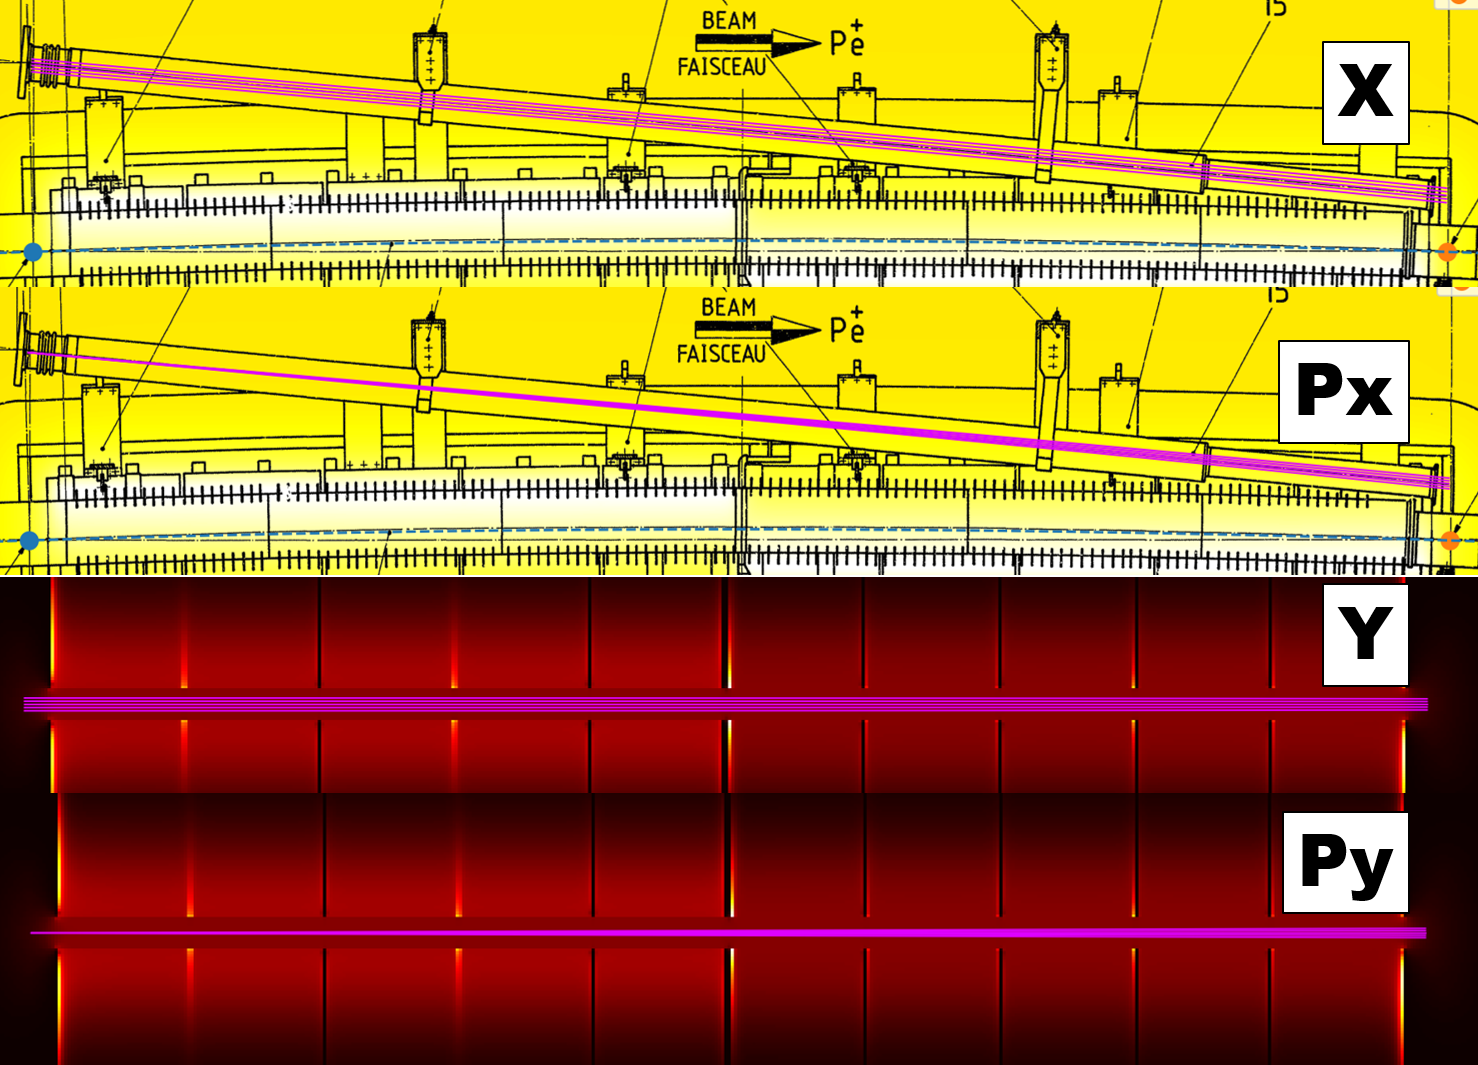
\includegraphics[width=1.0\textwidth]{02_Simulation/images/injection_transfer_matrix_3.png}
\caption{Particles are launched with different offsets.}
\label{fig:transfer_matrix_3}
\end{figure}

Figure \ref{fig:transfer_matrix_4} shows the transfer matrix points between the start and the end of the tracking inside the main unit. A linear fit is used to calculate the slope.

\begin{figure}[H]
\centering
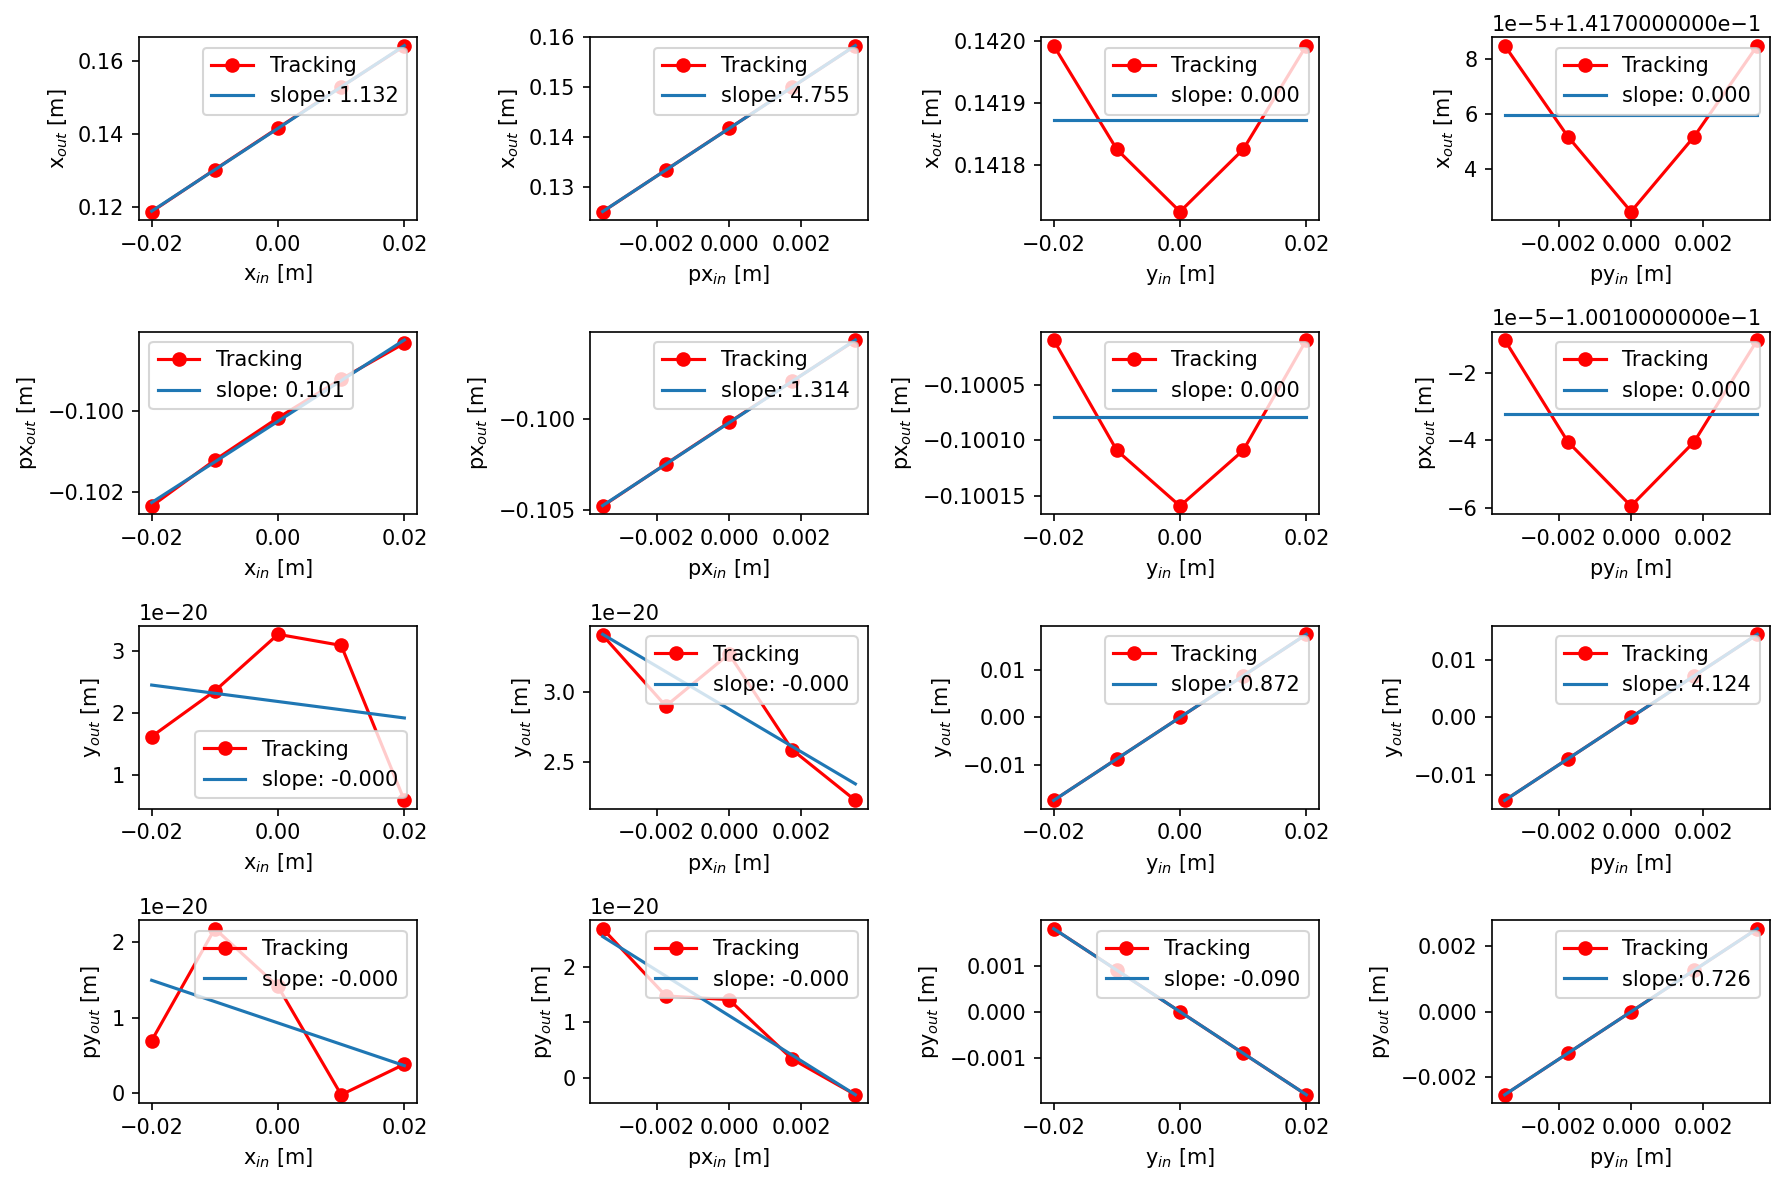
\includegraphics[width=1.0\textwidth]{02_Simulation/images/injection_transfer_matrix_4.png}
\caption{Particles are launched with different offsets.}
\label{fig:transfer_matrix_4}
\end{figure}



\textbf{Matrix from Tracking:}
\[
\begin{bmatrix}
1.132 & 4.755 & 0 & 0 \\
0.101 & 1.314 & 0 & 0 \\
0 & 0 & 0.872 & 4.124 \\
0 & 0 & -0.090 & 0.726
\end{bmatrix}
\]

The transfer matrix can also be visualized using color maps and compared to another transfer matrix tool developed by Ewa (called tracks.get\_transport\_matrix(k = k\_last, ret = 'mat')). Ewa's method eliminates the need for computationally intensive tracking. Instead, the nominal tracking can be used in conjunction with Ewa's function. However, it is important to note that this approach is only valid for the tracking section and does not extend to the SEM-Grid.

\begin{figure}[H]
\centering
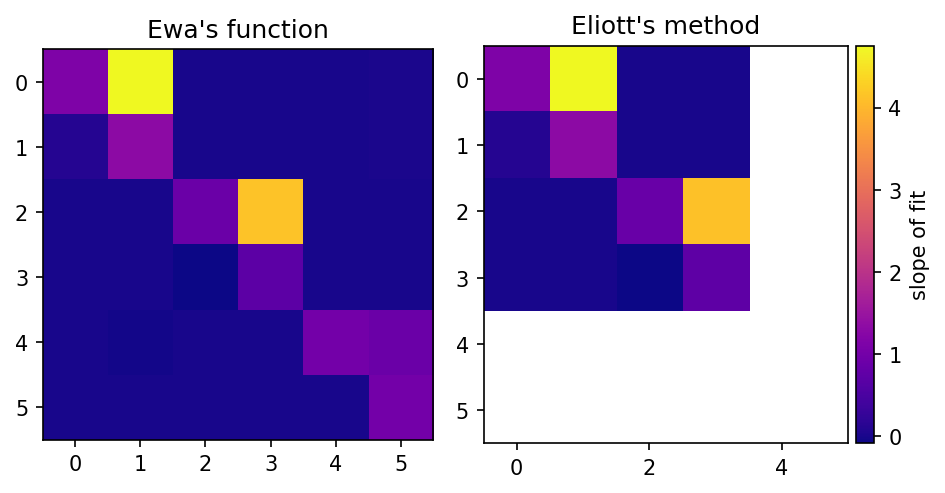
\includegraphics[width=1.0\textwidth]{02_Simulation/images/transfer_matrix_color.png}
\caption{Comparison between the matrix found by tracking at different offsets and Ewa's function.}
\label{fig:transfer_matrix_color}
\end{figure}





A transfer matrix, see Fig. \ref{fig:transfer_matrix_color}, can also be built as a function of POPS (from \si{500} to \si{1500}{gauss}) where it is observed that the injection angles are very sensitive to POPS change. The transfer matrix shows that injection angles are twice the sensitivity compared to horizontal (\(x\)) or vertical (\(y\)) offsets. This implies that any increase in POPS will significantly amplify the effect of a change in the horizontal angle (\(p_x\)) on the horizontal offset (\(x\)). Specifically, the matrix elements \(R_{21}\) and \(R_{22}\) exhibit the most substantial positive changes, indicating a strong correlation between \(p_{x,\text{in}}\) and both \(x_{\text{out}}\) and \(p_{x,\text{out}}\). Conversely, \(R_{34}\) and \(R_{44}\) show the most significant negative changes, highlighting the impact of \(p_{y,\text{in}}\) on both \(y_{\text{out}}\) and \(p_{y,\text{out}}\). These findings underscore the critical influence of POPS variations on beam dynamics, particularly in relation to injection angles.

\begin{figure}[H]
\centering
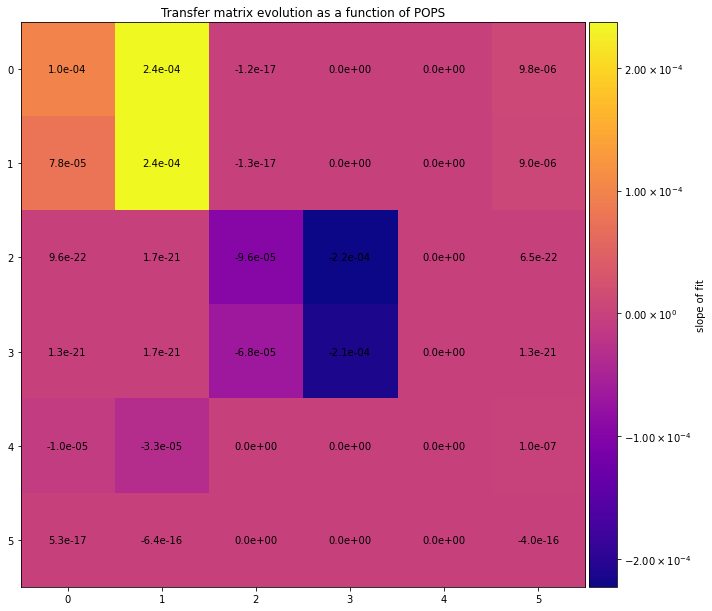
\includegraphics[width=1.0\textwidth]{02_Simulation/images/transfer_matrix_POPS.png}
\caption{Transfer matrix evolution as a function of POPS}
\label{fig:transfer_matrix_pops}
\end{figure}

The established transfer matrices can be utilized in MAD-X simulations to predict beam sizes under varying conditions. Notably, the elements \(R_{21}\), \(R_{22}\) (corresponding to \(p_{x,in}/x_{out}\) and \(p_{x,in}/p_{x,out}\)), and \(R_{34}\), \(R_{44}\) (corresponding to \(p_{y,in}/y_{out}\) and \(p_{y,in}/p_{y,out}\)) exhibited the most significant changes with variations in POPS, underscoring their critical role in beam dynamics at injection.


The source code for the simulations can be found in the following repositories:
\begin{itemize}
  \item \href{https://gitlab.cern.ch/eljohnso/acc-models-tls-eliott-fork/-/blob/EliottBranch/ps_injection/kick_response_injection_tracking/kick_response_BTP_injection_loop_transfer_matrix.ipynb}{Notebook: kick response BTP injection loop transfer matrix}
  \item \href{https://gitlab.cern.ch/eljohnso/acc-models-tls-eliott-fork/-/blob/EliottBranch/ps_injection/kick_response_injection_tracking/kick_response_BTP_injection_loop_transfer_matrix_function_of_POPS.ipynb}{Notebook: kick response BTP injection loop transfer matrix function of POPS.ipynb}
\end{itemize}


\subsection{Talk about how the shims are not implemented in OPERA and the solution in MAD-X}

\subsection{New chapter on extraction in F16}